\documentclass[11pt]{article}
\usepackage[T1]{fontenc}
\usepackage[utf8]{inputenc}
\usepackage{geometry}
%\geometry{letterpaper,landscape}
\geometry{paperwidth=9in,paperheight=7in}
%\usepackage{hyperref}
\usepackage[pdftex,
            pdfauthor={Bruno Ruviaro},
            pdftitle={Uma Gentil Introdução ao SuperCollider},
            pdfsubject={tutorial de SuperCollider},
            pdfkeywords={computação musical, SuperCollider, programação, música},
            pdfproducer={LaTeX},
            pdfcreator={pdflatex}]{hyperref}
            
\usepackage{enumerate}
\usepackage{graphicx}
\usepackage{endnotes}
\usepackage{listings}

\usepackage{listings}
\lstset{%
        inputencoding=utf8,
        extendedchars=true,
        literate=%
        {é}{{\'{e}}}1
        {è}{{\`{e}}}1
        {ê}{{\^{e}}}1
        {ë}{{\¨{e}}}1
        {É}{{\'{E}}}1
        {Ê}{{\^{E}}}1
        {û}{{\^{u}}}1
        {ú}{{\'{u}}}1
        {â}{{\^{a}}}1
        {à}{{\`{a}}}1
        {á}{{\'{a}}}1
        {ã}{{\~{a}}}1
        {Á}{{\'{A}}}1
        {Â}{{\^{A}}}1
        {Ã}{{\~{A}}}1
        {ç}{{\c{c}}}1
        {Ç}{{\c{C}}}1
        {õ}{{\~{o}}}1
        {ó}{{\'{o}}}1
        {ô}{{\^{o}}}1
        {Õ}{{\~{O}}}1
        {Ó}{{\'{O}}}1
        {Ô}{{\^{O}}}1
        {î}{{\^{i}}}1
        {Î}{{\^{I}}}1
        {í}{{\'{i}}}1
        {Í}{{\~{Í}}}1
}

\usepackage[symbol*, perpage]{footmisc}
\usepackage[colorinlistoftodos]{todonotes}
\usepackage[framed, numbered]{sclang-prettifier}
\renewcommand{\lstlistingname}{Example}
\title{\textbf{A Gentle Introduction to SuperCollider}}
\author{Bruno Ruviaro}
\usepackage[yyyymmdd]{datetime}
\renewcommand{\dateseparator}{-}
\date{\today}
%\DeclareUnicodeCharacter{0177}{\^y}
\usepackage[brazilian]{babel}

\begin{document}

% This is the first page, just title, no page number
\topskip0pt
\vspace*{\fill}
\begin{center}
{\LARGE \textbf{Uma Gentil Introdução ao SuperCollider}}

\bigskip
por Bruno Ruviaro

\medskip
revisão \today

tradução: Rodolfo Valente e Bruno Ruviaro


\bigskip
\bigskip

\begin{figure}[h]
\begin{center}
\includegraphics[scale=1]{fig-by-sa.png}
\end{center}
\end{figure}

\bigskip
Esta obra é disponibilizada sob a licença Creative Commons

Attribution-ShareAlike 4.0 International License.

Para ler uma cópia desta licença, visite:

\url{http://creativecommons.org/licenses/by-sa/4.0/}.



\end{center}
\vspace*{\fill}
\thispagestyle{empty}
\clearpage

% This is the table of contents
\pagenumbering{roman}
\tableofcontents
\maketitle
\pagenumbering{arabic}

\renewcommand{\partname}{Parte}
\renewcommand{\figurename}{Figura}

% This is the body of the text
% Page numbers are reset to arabic

% PART I
\part{O BÁSICO}
\section{Hello World}

Ready for creating your first SuperCollider program? Assuming you have SC up and running in front of you, open a new document (menu File$\rightarrow$New, or shortcut [ctrl+N]) and type the following line:

 
\begin{lstlisting}[style=SuperCollider-IDE, basicstyle=\scttfamily\footnotesize ]
"Hello World".postln;
\end{lstlisting}
 

Leave your cursor anywhere in that line (it doesn't matter if beginning, middle, or end). Press [ctrl+Enter] to evaluate the code. ``Hello world'' appears in the Post window. Congratulations! That was your first SuperCollider program.

 
\bigskip
\todo[inline, color=green!40]{ TIP: Throughout this document, ctrl (control) indicates the modifier key for keyboard shortcuts that is used on Linux and Windows platforms. On Mac OSX, use cmd (command) instead. }
\bigskip
 

Figure \ref{fig:scidegui} shows a screenshot of the SuperCollider IDE (Integrated Development Environment) when you first open it. Let's take a moment to get to know it a bit.

\begin{figure}[t]
\centerline{\framebox{
	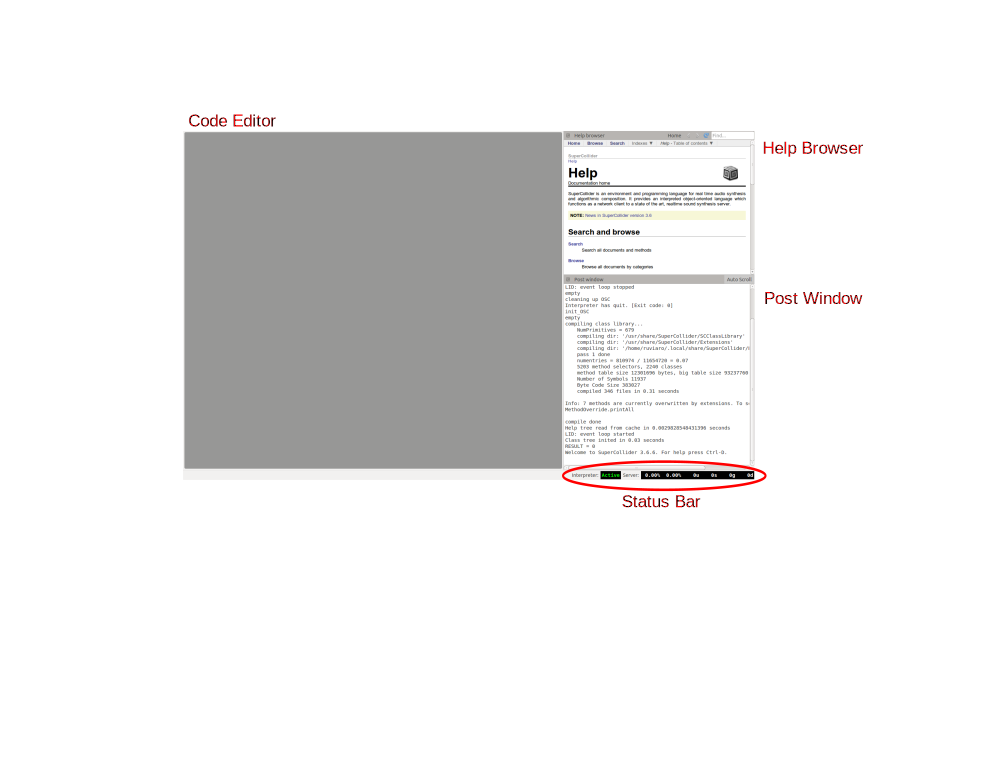
\includegraphics[width=0.7\columnwidth]{fig-supercollider-ide-2.png}}}
\caption{SuperCollider IDE interface.}
\label{fig:scidegui}
\end{figure}

What is the SuperCollider IDE? It is ``a cross-platform coding environment developed specifically for SuperCollider (\dots), easy to start using, handy to work with, and sprinkled with powerful features for experienced coders. It is also very customizable. It runs equally well and looks almost the same on Mac OSX, Linux and Windows.''\footnote{Quoted from the SuperCollider Documentation: \url{http://doc.sccode.org/Guides/SCIde.html}. Visit that page to learn more about the IDE interface.}

The main parts you see on the SC window are the Code Editor, the Help Browser, and Post Window. If you don't see any of these when you open SuperCollider, simply go to the menu View$\rightarrow$Docklets (that's where you can show or hide each of them). There is also the Status Bar, always located on the bottom right corner of the window.

Always keep the Post window visible, even if you don't understand yet all the stuff being printed there. The Post window displays the responses of the program to our commands: results of code evaluation, various notifications, warnings, errors, etc.

\bigskip
\todo[inline, color=green!40]{ TIP: You can temporarily enlarge and reduce the editor font size with the shortcuts [Ctrl++] and [Ctrl+-] (that's the control key together with the plus or minus keys, respectively). If you are on a laptop without a real plus key, use [Ctrl+shift+=].}
\bigskip



\section{Server and Language}

On the Status Bar you can see the words ``Interpreter'' and ``Server.'' The Interpreter starts up turned on by default (``Active''), while ``Server'' is turned off (that's what all the zeros  mean). What is the Interpreter, and what is the Server?

SuperCollider is actually made of two distinct applications: the server and the language. The server is responsible for making sounds. The language (also referred to as \emph{client} or \emph{interpreter}) is used to control the server. The first is called scsynth (SC-synthesizer), the second sclang (SC-language). The Status Bar tell us the status (on/off) of each one of these two components.

Don't worry if this distinction does not make much sense for you just now. The two main things you need to know at this point are:

\begin{enumerate}
\item Everything that you type in SuperCollider is in the SuperCollider language (the client): that's where you write and execute commands, and see results in the Post window.
\item Everything that makes sound in SuperCollider is coming from the server---the ``sound engine'', so to speak---, controlled by you through the SuperCollider language.
\end{enumerate}

\subsection{Booting the Server}
Your ``Hello World'' program produced no sound: everything happened in the language, and the server was not used at all. The next example will make sound, so we need to make sure the Server is up and running.

The easiest way to boot the server is with the shortcut [ctrl+B]. Alternatively, you can also click on the zeros in the Status Bar: a menu pops up, and one of the options is ``Boot Server.'' You will see some activity in the Post window as the server boots up. After you have successfully started the server, the numbers on the Status Bar will turn green. You will have to do this each time you launch SC, but only once per session.



\section{Sua primeira senóide \label{sec:first-sine}}


"Olá, Mundo" é tradicionalmente o primeiro programa que as pessoas criam quando estão aprendendo uma nova linguagem de programação. Você já fez isso no SuperCollider.

Criar uma onda senoidal simples talvez seja o "Olá, Mundo" das linguagens de programação para música. Vamos direto à senóide então. Digite e execute a seguinte linha de código. Cuidado---o volume pode ser alto. Abaixe todo seu volume do computador, execute a linha e aumente o volume devagar.
 
\begin{lstlisting}[style=SuperCollider-IDE, basicstyle=\scttfamily\footnotesize]
{SinOsc.ar}.play;
\end{lstlisting}
 

Trata-se de uma senoide bela, suave, contínua e talvez um pouco entediante. Você pode parar o som com [ctrl+.] (ou seja, a tecla \emph{control} junto com a tecla de \emph{ponto final}.) Memorize esta combinação de teclas, porque você a utilizará muito para interromper todo e qualquer som no SC.

\bigskip
\todo[inline, color=green!40]{ 
DICA: Em uma linha separada, digite e execute \texttt{s.volume.gui} se você quiser um slider gráfico para controlar o volume da saída do SuperCollider.
}
\bigskip

Agora vamos tornar esta senoide um pouco mais interessante. Digite isto:

 
\begin{lstlisting}[style=SuperCollider-IDE, basicstyle=\scttfamily\footnotesize ]
{SinOsc.ar(LFNoise0.kr(10).range(500, 1500), mul: 0.1)}.play;
\end{lstlisting}
 

Lembre-se, basta deixar o cursor em qualquer lugar da linha e apertar [ctrl+Enter] para executar. Ou, se preferir, você pode também selecionar toda a linha antes de executá-la.

 
\bigskip
\todo[inline, color=green!40]{ 
DICA: Digitar os próprios exemplos é uma grande ferramenta de aprendizagem. Isso irá ajudar a criar confiança e familiaridade com a linguagem. Ao ler tutoriais em formato digital, você pode às vezes sentir uma certa preguiça e ser tentado a copiar e colar o código dos exemplos. Evite fazer isso: você aprenderá melhor se digitar tudo por conta própria, ao menos nos primeiros estágios da sua aprendizagem com o SC.
}

\section{Mensagens de erro}

Não saiu nenhum som quando você rodou o último exemplo? Se isso aconteceu, provavelemente seu código tem um erro de digitação: um caracter errado, uma vírgula ou um parêntese a menos, etc. Quando algo acontece de errado no seu código, a Post window mostra uma mensagem de erro. Mensagens de erro podem ser longas e obscuras, mas não entre em pânico: com o tempo você aprenderá a lê-las. Veja abaixo um exemplo de uma mensagem de erro curta:

\begin{verbatim}
ERROR: Class not defined.
  in file 'selected text'
  line 1 char 19:

  {SinOsc.ar(LFNoiseO.kr(12).range(400, 1600), mul: 0.01)}.play; 
                     
-----------------------------------
nil
\end{verbatim}

Esta mensagem de erro diz "Class not defined" (Classe não definida) e aponta a localização aproximada do erro ("line 1 char 19", ou seja: linha 1, caracter 19). Classes no SC são aquelas palavras azuis que começam com uma letra maiúscula (como \texttt{SinOsc} e \texttt{LFNoise0}). O que causou o erro nesse exemplo foi que a pessoa digitou LFNoiseO com uma letra "O" maiúscula ao final. A classe correta é LFNoise0, com o número zero ao final. Parece até pegadinha de vestibular, mas é verdade. Como você pode ver, atenção aos detalhes é crucial.

Se você tem um erro no seu código, revise-o, mude o que for necessário e tente novamente até que ele esteja corrigido. Se você ainda não cometeu nenhum erro, experimente introduzir um para que você possa ver como é uma mensagem de erro (por exemplo, remova um ponto ou uma vírgula de um dos exemplos das senoides).

\bigskip
\todo[inline, color=green!40]{ 
DICA: Aprender SuperCollider é como aprender uma outra língua como Alemão, Inglês ou Japonês\dots\  você tem que praticar falá-la o máximo possível, esforce-se em expandir seu vocabulário, preste atenção na gramática e na sintaxe e aprenda com seus erros. A pior coisa que pode acontecer é você travar o SuperCollider, o que é bem menos ruim do que pegar um ônibus errado em Nova Iorque por culpa de um erro de pronúncia na hora de pedir informações.
}

\section{Mudando parâmetros}

Segue abaixo um exemplo interessante adaptado do primeiro capítulo do The SuperCollider Book.\footnote{
Wilson, S. and Cottle, D. and Collins, N. (Editors). The SuperCollider Book, MIT Press, 2011, p. 5. Diversas coisas neste tutorial foram emprestadas, adaptadas ou inspiradas pelo excelente "Beginner’s Tutorial" de David Cottle, que é o primeiro capítulo do livro, mas---diferentemente dele--aqui assumimos que o leitor tenha pouca familiaridade com computação musical, e apresentamos a família de Patterns como eixo principal da abordagem pedagógica.
} Da mesma forma que em exemplos anteriores, não se preocupe em entender tudo. Apenas aprecie o resultado sonoro e brinque com os números.


\begin{lstlisting}[style=SuperCollider-IDE, basicstyle=\scttfamily\footnotesize]
{RLPF.ar(Dust.ar([12, 15]), LFNoise1.ar([0.3, 0.2]).range(100, 3000), 0.02)}.play;
\end{lstlisting}

Pare o som, mude alguns números e rode novamente. Por exemplo, o que acontece quando você substitui os números 12 e 15 por valores mais baixos, entre 1 e 5? Depois de \texttt{LFNoise1}, que tal se em vez de 0.3 e 0.2 você tentasse algo como 1 ou 2? Mude um de cada vez. Compare o novo som com o som anterior, escute as diferenças. Veja se você consegue entender qual número está controlando o quê. Esta é uma maneira divertida de explorar o SuperCollider: pegue um trecho de código que faça algo interessante e experimente com os parâmetros para criar variações. Mesmo se você não entender completamente a função exata de cada número, ainda assim pode encontrar resultados sonoros interessantes.

\bigskip 
\todo[inline, color=green!40]{ 
DICA: Como qualquer software, lembre-se de salvar frequentemente o seu trabalho com [ctrl+S]! Quanto estiver trabalhando em tutoriais como esse, você muitas vezes vai chegar a sons interessantes experimentando com os exemplos fornecidos. Quando você quiser guardar algo que gostou, copie o código em um novo documento e salve-o. Repare que todo arquivo do SuperCollider tem a extensão .scd, que quer dizer "SuperCollider Document."
}

\section{Comentários}

Todo o texto que aparece em vermelho no seu código é um \emph{comentário}. Se você é novo em linguagens de programação, comentários são bastante úteis para documentar o seu código, tanto para você mesmo, quanto para outros que tenham de lê-lo depois. Qualquer linha começando com uma barra dupla é um comentário. Você pode escrever comentários logo depois de uma linha válida de código, pois a parte do comentário será ignorada quando você rodar. No SC, usamos um ponto-e-vírgula para indicar o fim de um enunciado válido.

\begin{lstlisting}[style=SuperCollider-IDE, basicstyle=\scttfamily\footnotesize]
2 + 5 + 10 - 5; // apenas fazendo contas

rrand(10, 20); // gerar um numero aleatório entre 10 e 20
\end{lstlisting}

Você pode rodar uma linha mesmo que o seu cursor estiver no meio de um comentário depois desta linha. A parte do comentário é ignorada. Os próximos dois parágrafos serão escritos como "comentários" apenas como exemplo.


 
\begin{lstlisting}[style=SuperCollider-IDE, basicstyle=\scttfamily\footnotesize]
// Você pode rapidamente transformar uma linha de código em comentário usando o atalho [ctrl+/].
"Algum código de SC aqui...".postln;
2 + 2;


// Se você escrever um comentário beeeem longo (uma única linha longa), seu texto vai ser quebrado em várias "linhas" que não vão começar com barra dupla. No entanto, tudo isso ainda conta como uma só linha de comentário.

/* Use "barra + asterisco" para começar um comentário longo com diversas linhas. Feche o trecho de comentário com "asterisco + barra". O atalho mencionado anteriormente também funciona para grandes trechos: simplesmente selecione as linhas de código que você quer "comentar" ("comment out", em inglês) e pressione [ctrl+/]. O mesmo serve para des-comentar ("uncomment").*/
\end{lstlisting}

\section{Precedência}

O SuperCollider segue a ordem de precedência da esquerda para a direita, independente da operação. Isso significa, por exemplo, que multiplicação \emph{não} acontece primeiro:

\begin{lstlisting}[style=SuperCollider-IDE, basicstyle=\scttfamily\footnotesize]
// No colégio, o resultado era 9; no SC é 14:
5 + 2 * 2; 
//Use parênteses para forçar uma ordem de operações específica:
5 + (2 * 2); // igual a 9.
\end{lstlisting}

Quando se combina mensagens e operações binárias, mensagens assumem precedência. Por exemplo, em \texttt{5 + 2.squared}, a elevação ao quadrado acontece primeiro.

\section{The last thing always gets posted}

A small but useful detail to understand: SuperCollider, by default, always posts to the Post window the result of whatever was the \emph{last thing to be evaluated}. This explains why your Hello World code prints twice when you evaluate. Type the following lines onto a new document, then select all with [ctrl+A] and evaluate all lines at once:

\begin{lstlisting}[style=SuperCollider-IDE, basicstyle=\scttfamily\footnotesize]
"First Line".postln;
"Second Line".postln;
(2 + 2).postln;
3 + 3;
"Finished".postln;
\end{lstlisting}

All five lines are executed by SuperCollider. You see the result of \texttt{2 + 2} in the Post window because there was an explicit \texttt{postln} request. The result of \texttt{3 + 3} was calculated, but there was no request to post it, so you don't see it. Then the command of the last line is executed (the word ``Finished'' gets posted due to the \texttt{postln} request). Finally, the result of the very last thing to be evaluated is posted by default: in this case, it happened to be the word ``Finished.''
\section{Blocos de código}
\label{sec:code-block}


Selecionando múltiplas linhas de um código antes de rodá-lo pode ser tedioso. Uma maneira muito mais fácil de rodar toda uma porção de código ao mesmo tempo é criar um \textit{bloco de código}: simplesmente coloque dentro de parênteses todas as linhas de código que você quer rodar juntas. Aqui temos um exemplo:


\begin{lstlisting}[style=SuperCollider-IDE, basicstyle=\scttfamily\footnotesize]
(
// Um pequeno poema
“Hoje é domingo“.postln;
“Pé de cachimbo”.postln;
“O cachimbo é de ouro”.postln;
“Bate no touro”.postln;
)
\end{lstlisting}

Os parênteses externos delimitam o bloco de código. Desde que que o cursor esteja em qualquer lugar dentro dos parênteses, um único [ctrl+Enter] rodará as linhas para você (elas serão executadas na ordem de cima para baixo, mas isso é tão rápido que parece simultâneo).

Usar blocos de código poupa o trabalho de ter de selecionar todas as linhas novamente a cada vez que você quiser mudar algo e rodar novamente. Por exemplo mude algumas das palavras entre aspas e pressione [ctrl+Enter] logo após fazer a mudança. Todo o bloco de código é rodado sem que você tenha que selecionar manualmente todas as linhas. O SuperCollider ressalta o bloco por um segundo para dar uma indicação visual de o que está sendo executado.

\section{Como limpar a Post window}

Este é um comando tão útil para maníacos por limpeza que merece uma seção só pra ele: [ctrl+shift+P]. Execute esta linha e experimente limpar a Post window em seguida:

 
\begin{lstlisting}[style=SuperCollider-IDE, basicstyle=\scttfamily\footnotesize]
100.do({"Imprima esta linha um monte de vezes...".scramble.postln});
\end{lstlisting}
 
Não precisa agradecer.


\section{Recording the output of SuperCollider}

Soon you will want to start recording the sound output of your SuperCollider patches. Here's a quick way:
 
\begin{lstlisting}[style=SuperCollider-IDE, basicstyle=\scttfamily\footnotesize]
// QUICK RECORD
// Start recording:
s.record;
// Make some cool sound
{Saw.ar(LFNoise0.kr([2, 3]).range(100, 2000), LFPulse.kr([4, 5]) * 0.1)}.play;
// Stop recording:
s.stopRecording;
// Optional: GUI with record button, volume control, mute button:
s.makeWindow;
\end{lstlisting}
 
The Post Window shows the path of the folder where the file was saved. Find the file, open it with Audacity or similar program, and verify that the sound was indeed recorded. For more info, look at the ``Server'' Help file (scroll down to ``Recording Support''). Also online at \url{http://doc.sccode.org/Classes/Server.html}.
\section{Variables}
\label{sec:variables}

You can store numbers, words, unit generators, functions, or entire blocks of code in variables. Variables can be single letters or whole words chosen by you. We use the equal sign (=) to ``assign'' variables. Run these lines one at a time and watch the Post window:

 
\begin{lstlisting}[style=SuperCollider-IDE, basicstyle=\scttfamily\footnotesize]
x = 10;
y = 660;
y; // check what's in there
x;
x + y;
y - x;
\end{lstlisting}
 

The first line assigns the number 10 to the variable \texttt{x}. The second line puts 660 into the variable \texttt{y}. The next two lines prove that those letters now ``contain'' those numbers (the data). Finally, the last two lines show that we can use the variables to do any operations with the data.

Lowercase letters \texttt{a} through \texttt{z} can be used anytime as variables in SuperCollider. The only single letter that by convention we don't use is \texttt{s}, which by default represents the Server. Anything can go into a variable:
 
\begin{lstlisting}[style=SuperCollider-IDE, basicstyle=\scttfamily\footnotesize]
a = "Hello, World"; // a string of characters
b = [0, 1, 2, 3, 5]; // a list
c = Pbind(\note, Pwhite(0, 10), \dur, 0.1); // you'll learn all about Pbind later, don't worry

// ...and now you can use them just like you would use the original data:
a.postln; // post it
b + 100; // do some math
c.play; // play that Pbind
d = b * 5; // take b, multiply by 5, and assign that to a new variable
\end{lstlisting}

Often it will make more sense to give better names to your variables, to help you remember what they stand for in your code. You can use a $\sim$ (tilde) to declare a variable with a longer name. Note that there is no space between the tilde and the name of the variable.

\begin{lstlisting}[style=SuperCollider-IDE, basicstyle=\scttfamily\footnotesize]
~myFreqs = [415, 220, 440, 880, 220, 990];
~myDurs = [0.1, 0.2, 0.2, 0.5, 0.2, 0.1];

Pbind(\freq, Pseq(~myFreqs), \dur, Pseq(~myDurs)).play;
\end{lstlisting}
 

Variable names must begin with lowercase letters. You can use numbers, underscores, and uppercase letters within the name, just not as the first character. All characters must be contiguous (no spaces or punctuation). In short, stick to letters and numbers and the occasional underscore, and avoid all other characters when naming your variables. \texttt{$\sim$myFreqs}, \texttt{$\sim$theBestSineWave}, and \texttt{$\sim$banana\_3} are valid names. \texttt{$\sim$MyFreqs}, \texttt{$\sim$theBest\&*\#\@SineWave}, and \texttt{$\sim$banana!!!} are bad names.

There are two types of variables that you can create: ``global'' variables and local variables.

\subsection{``Global'' vs. Local}

The variables you have seen up to now (the single lowercase letters \texttt{a} through \texttt{z}, and those starting with the tilde ($\sim$) character) may be loosely called ``global variables,'' because once declared, they will work ``globally'' anywhere in the patch, in other patches, even in other SC documents, until you quit SuperCollider.\footnote{Technically speaking, variables starting with a tilde are called Environment variables, and lowercase letter variables (a through z) are called Interpreter variables. SuperCollider beginners do not need to worry about these distinctions, but keep them in mind for the future. Chapter 5 of the SuperCollider book explains the differences in detail.}

Local variables, on the other hand, are declared with the reserved keyword \texttt{\textbf{var}} at the beginning of the line. You can assign an initial value to a variable at declaration time (\texttt{\textbf{var} apples = 4}). Local variables only exist within the scope of that code block.

Here's a simple example comparing the two types of variables. Evaluate line by line and watch the Post window.

 
\begin{lstlisting}[style=SuperCollider-IDE, basicstyle=\scttfamily\footnotesize]
// Environment variables
~galaApples = 4;
~bloodOranges = 5;
~limes = 2;
~plantains = 1;

["Citrus", ~bloodOranges + ~limes];
["Non-citrus", ~plantains + ~galaApples];

// Local variables: valid only within the code block.
// Evaluate the block once and watch the Post window:
(
var apples = 4, oranges = 3, lemons = 8, bananas = 10;
["Citrus fruits", oranges + lemons].postln;
["Non-citrus fruits", bananas + apples].postln;
"End".postln;
)

~galaApples; // still exists
apples; // gone
\end{lstlisting}

\subsection{Reassignment}

One last useful thing to understand about variables is that they can be \emph{reassigned}: you can give them a new value at anytime.

\begin{lstlisting}[style=SuperCollider-IDE, basicstyle=\scttfamily\footnotesize]
// Assign a variable
a = 10 + 3;
a.postln; // check it
a = 999; // reassign the variable (give it a new value)
a.postln; // check it: the old value is gone.
\end{lstlisting}

A very common practice that is sometimes confusing for beginners is when \emph{the variable itself is used in its own reassignment}. Take a look at this example:

\begin{lstlisting}[style=SuperCollider-IDE, basicstyle=\scttfamily\footnotesize]
x = 10; // assign 10 to the variable x
x = x + 1; // assign x + 1 to the variable x
x.postln; // check it
\end{lstlisting}

The easiest way to understand that last line is to read it like this: ``take the current value of variable x, add 1 to it, and assign this new result to the variable x.'' It's really not complicated, and you will see later on how this can be useful.\footnote{This example clearly demonstrates that the equal sign, in programming, is not the same equal sign that you learned in mathematics. In math, $x = x + 1$ is impossible (a number cannot be equal to itself plus one). In a programming language like SuperCollider, the equal sign can be seen as a kind of action: \emph{take the result of the expression on the right side of the sign, and ``assign it'' to the variable on the left side}.}
% PART II
\newpage
\part{PATTERNS}
\section{A família Pattern}

Vamos experimentar algo diferente agora. Digite e rode esta linha de código:

\begin{lstlisting}[style=SuperCollider-IDE, basicstyle=\scttfamily\footnotesize]
Pbind(\degree, Pseries(0, 1, 30), \dur, 0.05).play;
\end{lstlisting}

\subsection{Conheça o Pbind}

\texttt{Pbind} é um membro da família Pattern ("padrão" ou "modelo") no SuperCollider. O P maiúsculo no \texttt{Pbind} e \texttt{Pseries} remete a \emph{Pattern}; em breve teremos o prazer de conhecer outros membros da família. Por ora, vamos focar somente somente no \texttt{Pbind}. Experimente este exemplo reduzido ao mínimo:

\begin{lstlisting}[style=SuperCollider-IDE, basicstyle=\scttfamily\footnotesize]
Pbind(\degree, 0).play;
\end{lstlisting}

A única coisa que esta linha de código faz na vida é tocar a nota \emph{dó central}, uma vez por segundo. A palavra-chave \texttt{\textbackslash degree} se refere a graus de uma escala e o número 0 representa o primeiro grau da escala (uma escala de Dó Maior é subentendida, então esta é a própria nota dó). Note que o SuperCollider começa a contar as coisas do 0 e não do 1. Em uma linha simples como esta acima, as notas dó, ré, mi, fá, sol\dots seriam representadas pelos números 0, 1, 2, 3, 4\dots Tente mudar o número e perceba como a nota muda quando você reexecuta. Você também pode escolher notas abaixo do dó central (por exemplo, -2 é a nota lá abaixo do dó central). Resumindo, apenas imagine que o dó central do piano é 0 e conte teclas brancas para cima ou para baixo (números positivos ou negativos) para obter qualquer outra nota.

Agora brinque um pouco com a duração das notas. \texttt{Pbind} usa a palavra-chave \texttt{\textbackslash dur} para especificar durações em segundos:

\begin{lstlisting}[style=SuperCollider-IDE, basicstyle=\scttfamily\footnotesize]
Pbind(\degree, 0, \dur, 0.5).play;
\end{lstlisting}

Claro que isso ainda é muito rígido e inflexível---sempre a mesma nota, sempre a mesma duração. Não se preocupe: as coisas vão esquentar logo, logo.
\subsection{Pseq}

Vamos agora tocar várias notas em sequência, como uma escala. Vamos também diminuir a duração das notas para 0.2 segundos.
 
\begin{lstlisting}[style=SuperCollider-IDE, basicstyle=\scttfamily\footnotesize]
Pbind(\degree, Pseq([0, 1, 2, 3, 4, 5, 6, 7], 1), \dur, 0.2).play;
\end{lstlisting}

Esta linha introduz um novo membro da família Pattern: \texttt{Pseq}. Como o nome sugere, este Pattern lida com sequências. Tudo que um \texttt{Pseq} precisa para tocar uma sequência é:
\begin{itemize}
\item uma lista de itens entre colchetes []
\item um número de repetições.
\end{itemize} 

No exemplo, a lista é \texttt{[0, 1, 2, 3, 4, 5, 6, 7]} e o número de repetições é \texttt{1}. Este \texttt{Pseq} simplesmente diz: "toque todos os itens da lista, na sequência, uma vez". Repare que estes dois elementos, lista e número de repetições, estão dentro dos parênteses que pertencem ao \texttt{Pseq} e são separados por uma vírgula.

Veja também onde o \texttt{Pseq} aparece no interior do \texttt{Pbind}: é colocado como valor de \texttt{\textbackslash degree}. Isso é importante: em vez de fornecer um número único e fixo para o grau da escala (como no nosso primeiro \texttt{Pbind} simples), \emph{estamos fornecendo todo um Pseq: uma receita para uma sequência de números}. Com isto em mente, podemos facilmente expandir esta ideia e usar outro Pseq para controlar também as durações.
 
\begin{lstlisting}[style=SuperCollider-IDE, basicstyle=\scttfamily\footnotesize]
Pbind(\degree, Pseq([0, 1, 2, 3, 4, 5, 6, 7], 5), \dur, Pseq([0.2, 0.1, 0.1, 0.2, 0.2, 0.35], inf)).play;
\end{lstlisting}
 
O que está acontecendo neste exemplo? Primeiro, mudamos o número de repetições do primeiro \texttt{Pseq} para 5, de modo que toda a escala vai tocar cinco vezes. Segundo, substituímos o valor de \texttt{\textbackslash dur}, antes fixo em 0.2, por um outro \texttt{Pseq}. Este novo \texttt{Pseq} tem uma lista de seis itens: \texttt{[0.2, 0.1, 0.1, 0.2, 0.2, 0.35]}. Estes números se tornam valores de duração das notas resultantes. O valor de \texttt{repeats} deste segundo \texttt{Pseq} é definido como \texttt{inf}, que quer dizer "infinito". Isso sgnifica que o \texttt{Pseq} não tem limite no número de vezes que ele pode repetir esta sequência. Então o \texttt{Pbind} toca para sempre? Não: ele para depois que o \emph{outro} \texttt{Pseq} terminou seu trabalho, isto é, depois que a sequência de graus de escala foi tocada 5 vezes.

Finalmente, o exemplo tem um total de oito notas diferentes (a lista no primeiro \texttt{Pseq}), enquanto há apenas seis valores para duração (segundo \texttt{Pseq}). Quando você fornece sequências de tamanhos diferentes como estas, o \texttt{Pbind} simplesmente as faz circular o quanto for preciso.

Responda estas perguntas para praticar o que você aprendeu:
\begin{itemize}
\item Experimente o número 1 em vez de inf como o argumento \texttt{repeats} do segundo \texttt{Pseq}. O que acontece?
\item Como você pode fazer este Pbind tocar para sempre?
\end{itemize}

Soluções estão no final do livro.\endnote{Primeira pergunta: quando você usa o número 1 em vez de \texttt{inf} como o argumento \texttt{repeats} do segundo \texttt{Pseq}, o Pbind para depois que 6 notas foram tocadas (isto é, depois que uma sequência completa de valores de duração foi tocada). Segunda questão: para fazer o Pbind tocar para sempre, simplesmente use \texttt{inf} como valor para \texttt{repeats} em todos os Patterns internos.}

\subsection{Deixe seu código mais legível}

Você deve ter percebido que a linha de código acima é um tanto longa. De fato, ela é tão longa que quebra em uma nova linha, mesmo que tecnicamente se trate de um enunciado único. Linhas de código longas podem ser confusas de ler. Para evitar isso, é uma prática comum quebrar o código em várias linhas indentadas; com o objetivo de torná-lo o mais claro e inteligível possível. O mesmo \texttt{Pbind} pode ser escrito assim:

\begin{lstlisting}[style=SuperCollider-IDE, basicstyle=\scttfamily\footnotesize]
(
Pbind(
	\degree, Pseq([0, 1, 2, 3, 4, 5, 6, 7], 5),
	\dur, Pseq([0.2, 0.1, 0.1, 0.2, 0.2, 0.35], inf)
).play;
)
\end{lstlisting}

De agora em diante, adquira o hábito de escrever seus \texttt{Pbind}s deste jeito. Escrever código com uma aparência arrumada e bem organizada vai ajudá-lo bastante no aprendizado do SuperCollider.

Além disso, perceba que envolvemos este \texttt{Pbind} dentro de parênteses para criar um bloco de código (lembra-se da seção \ref{sec:code-block}?): como ele não está mais em uma única linha, precisamos fazer isso para conseguir rodá-lo todo de uma vez. Lembre-se que o cursor precisa estar em algum lugar no interior do bloco antes de executá-lo.


\subsection{Quatro maneiras de especificar alturas}

\texttt{Pbind} aceita outras maneiras de especificar alturas, não apenas graus de escala.
\begin{itemize}
\item Se você quiser usar todas as doze notas cromáticas (teclas brancas e pretas do piano), você pode usar \texttt{\textbackslash note} em vez de \texttt{\textbackslash degree}. 0 continuará representando o dó central, mas agora os números incluem as teclas pretas do piano (0=dó central, 1=dó$\sharp$, 2=ré, etc).
\item Se você preferir usar a numeração de notas MIDI, use \texttt{\textbackslash midinote} (60=dó central, 61=dó$\sharp$, 62=ré, etc).
\item Finalmente, se você quiser especificar frequências diretamente em Herz, use \texttt{\textbackslash freq}.
\end{itemize}

Veja a figura \ref{fig:scale-degrees} para uma comparação dos quatro métodos.

\begin{figure}[h]
\centering
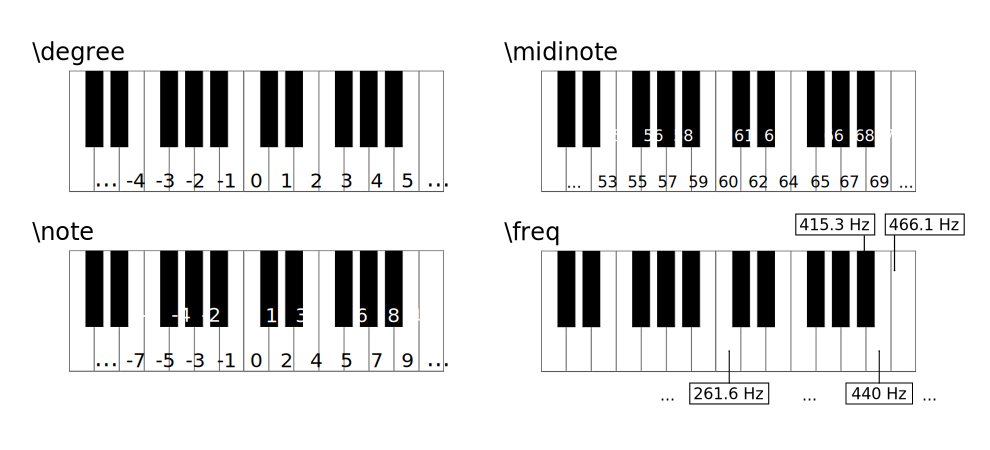
\includegraphics[scale=0.4]{fig-piano-keyboard-degree-note-midinote-freq.png}
\caption{Comparando graus de escala, números de nota, notas MIDI e frequências}
\label{fig:scale-degrees}
\end{figure}

No próximo exemplo, quatro Pbinds vão tocar a mesma nota: o lá acima do dó central (lá 4).

\begin{lstlisting}[style=SuperCollider-IDE, basicstyle=\scttfamily\footnotesize]
Pbind(\degree, 5).play;
Pbind(\note, 9).play;
Pbind(\midinote, 69).play;
Pbind(\freq, 440).play;
\end{lstlisting}


\bigskip
\todo[inline, color=green!40]{
DICA: Lembre-se que cada maneira de especificar alturas requer números em âmbitos dife-rentes. Uma lista de números como \texttt{[-1, 0, 1, 3]} faz sentido para \texttt{\textbackslash degree} e \texttt{\textbackslash note}, mas não faz sentido para \texttt{\textbackslash midinote} ou \texttt{\textbackslash freq}. A tabela abaixo compara alguns valores usando o teclado do piano como referência.
}
\bigskip


\begin{tabular}{|l|c|c|c|c|c|}
\hline 
  & \textbf{lá 0 (nota mais grave do piano)} & \textbf{dó 4} & \textbf{lá 4} & \textbf{dó 5} & \textbf{dó 8} \\ 
\hline 
\texttt{\textbackslash degree} & -23 & 0 & 5 & 7 & 21 \\
\hline
\texttt{\textbackslash note} & -39 & 0 & 9 & 12 & 48 \\
\hline
\texttt{\textbackslash midinote} & 21 & 60 & 69 & 72 & 108 \\
\hline
\texttt{\textbackslash freq} & 27.5 & 261.6 & 440 & 523.2 & 4186 \\
\hline
\end{tabular}
\bigskip


\subsection{Mais palavras-chave: amplitude e legato}

O novo exemplo introduz duas novas palavras-chave: \texttt{\textbackslash amp} e \texttt{\textbackslash legato}, que definem a amplitude dos eventos e a quantidade de legato entre as notas. Perceba como o código fica bem mais fácil de ler, graças a uma boa indentação e distribuição em várias linhas. Parênteses externos (no topo e embaixo) são usados para delimitar um bloco de código a ser executado de uma vez.

 
\begin{lstlisting}[style=SuperCollider-IDE, basicstyle=\scttfamily\footnotesize]
(
Pbind(
	\degree, Pseq([0, -1, 2, -3, 4, -3, 7, 11, 4, 2, 0, -3], 5),
	\dur, Pseq([0.2, 0.1, 0.1], inf),
	\amp, Pseq([0.7, 0.5, 0.3, 0.2], inf),
	\legato, 0.4
).play;
)
\end{lstlisting}
 

\texttt{Pbind} tem muitas destas palavras-chave pré-definidas e, com o tempo, você aprenderá mais delas. Por agora, vamos nos centrar em apenas algumas---uma para altura (com as opções de \texttt{\textbackslash degree}, \texttt{\textbackslash note}, \texttt{\textbackslash midinote} ou \texttt{\textbackslash freq}), uma para durações (\texttt{\textbackslash dur}), uma para amplitude (\texttt{\textbackslash amp}) e uma para legato (\texttt{\textbackslash legato}). Durações estão em tempos (neste caso, 1 batida por segundo, que é o padrão); a amplitude deve estar entre 0 e 1 (0 = silêncio, 1 = muito alto); e o legato funciona melhor com valores entre 0.1 e 1 (se você não tem certeza o que o legato faz, simplesmente experimente o exemplo acima com 0.1, depois 0.2, depois 0.3, até chegar no 1 e ouça os resultados).

Tome o último exemplo como um  ponto de partida e crie novos \texttt{Pbind}s. Mude a melodia. Introduza novas listas de durações e amplitudes. Experimente usar \texttt{\textbackslash freq} para alturas. Lembre-se, você sempre pode usar um número fixo para qualquer um destes parâmetros, se quiser. Por exemplo, se você quer que todas as notas da sua melodia tenham 0.2 segundos de duração, não há porque escrever \texttt{Pseq[0.2, 0.2, 0.2, 0.2\dots}, nem mesmo \texttt{Pseq([0.2], inf)}---simplesmente remova toda a estrutura do \texttt{Pseq} e escreva 0.2 no lugar.

\subsection{Prand}

\texttt{Prand} é um parente próximo do \texttt{Pseq}. Ele também aceita uma lista e um número de repetições. Mas em vez de ir tocando a lista na sequência, \texttt{Prand} \emph{escolhe um item aleatório da lista a cada vez}. Experimente:

 
\begin{lstlisting}[style=SuperCollider-IDE, basicstyle=\scttfamily\footnotesize]
(
Pbind(
	\degree, Prand([2, 3, 4, 5, 6], inf),
	\dur, 0.15,
	\amp, 0.2,
	\legato, 0.1
).play;
)
\end{lstlisting}
 

Substitua \texttt{Prand} pelo \texttt{Pseq} e compare os resultados. Agora experimente usar \texttt{Prand} para durações, amplitudes e legato.

\subsection{Pwhite}

Outro membro popular da família Pattern é o \texttt{Pwhite}. É um gerador de números aleatórios de distribuição uniforme (o nome vem de "white noise", ruído branco). Por exemplo, \texttt{Pwhite(100, 500)} irá fornecer números aleatórios entre 100 e 500.
 
\begin{lstlisting}[style=SuperCollider-IDE, basicstyle=\scttfamily\footnotesize]
(
Pbind(
	\freq, Pwhite(100, 500),
	\dur, Prand([0.15, 0.25, 0.3], inf),
	\amp, 0.2,
	\legato, 0.3
).trace.play;
)
\end{lstlisting}
 

O exemplo acima também mostra outro truque útil: a mensagem \texttt{trace} logo antes de \texttt{play}. Isso imprime na Post window os valores selecionados em cada evento. Muito útil para corrigir problemas ou simplesmente para entender o que está acontecendo!

Preste atenção nas diferenças entre \texttt{Pwhite} e \texttt{Prand}: mesmo que ambos tenham a ver com aleatoriedade, eles aceitam argumentos distintos e fazem coisas diferentes. Dentro dos parênteses do \texttt{Pwhite} você só precisa fornecer um limite mínimo e máximo: \texttt{Pwhite(mínimo, máximo)}. Números aleatórios serão escolhidos no interior deste âmbito. \texttt{Prand}, por outro lado, aceita uma lista de itens (necessariamente entre colchetes) e um número de repetições: \texttt{Prand([lista, de, itens], repetições)}. Itens aleatórios serão escolhidos \emph{desta lista}.

Explore ambos e confirme que você entendeu completamente a diferença.


\bigskip
\todo[inline, color=green!40]{ 
DICA: Um \texttt{Pwhite} com dois números inteiros vai gerar somente números inteiros. Por exemplo, \texttt{Pwhite(100, 500)} vai gerar números como 145, 568, 700, mas não 145.6, 450.32, etc. Se você quer incluir números decimais no resultado, escreva \texttt{Pwhite(100, 500.0)}. Isso é muito útil para, digamos, amplitudes: se você escreve \texttt{Pwhite(0, 1)} vai obter apenas 0 ou 1, mas escreva \texttt{Pwhite(0, 1.0)} e você terá todos os resultados intermediários.
}
\bigskip
 


Tente as seguintes perguntas para testar seu novo conhecimento:

\begin{enumerate}[a)]
\item Qual a diferença entre os resultados de \texttt{Pwhite(0, 10)} e \texttt{Prand([0, 4, 1, 5, 9, 10, 2, 3], inf)}?

\item Se você precisa de um fluxo de números inteiros escolhidos aleatoriamente entre 0 e 100, você poderia usar um \texttt{Prand}?

\item Qual a diferença entre os resultados de \texttt{Pwhite(0, 3)} e \texttt{Prand([0, 1, 2, 3], inf)}? E se você escrever \texttt{Pwhite(0, 3.0)}?

\item  Rode os exemplos abaixo. Usamos \texttt{\textbackslash note} em vez de \texttt{\textbackslash degree} para tocar uma escala de dó menor (que inclui teclas pretas). A lista \texttt{[0, 2, 3, 5, 7, 8, 11, 12]} tem oito números dentro dela, correspondendo às notas dó, ré, mi$\flat$, fá, sol, lá$\flat$, si, dó, mas quantos eventos cada exemplo realmente toca? Por quê?

 
\begin{lstlisting}[style=SuperCollider-IDE, basicstyle=\scttfamily\footnotesize]
// Pseq
(
Pbind(
	\note, Pseq([0, 2, 3, 5, 7, 8, 11, 12], 4),
	\dur, 0.15;
).play;
)

// Pseq
(
Pbind(
	\note, Prand([0, 2, 3, 5, 7, 8, 11, 12], 4),
	\dur, 0.15;
).play;
)

// Pwhite
(
Pbind(
	\note, Pseq([0, 2, 3, 5, 7, 8, 11, 12], 4),
	\dur, Pwhite(0.15, 0.5);
).play;
)
\end{lstlisting}

\end{enumerate}


Respostas ao final deste tutorial.\endnote{\\
a) \texttt{Pwhite(0, 10)} vai gerar qualquer número entre 0 e 10. \texttt{Prand([0, 4, 1, 5, 9, 10, 2, 3], inf)} vai escolher apenas números que estão contidos na lista; note que essa lista tem \emph{alguns} números entre 0 e 10, mas não todos (6, 7, 8 não estão lá, então nunca vão aparecer neste \texttt{Prand}).  \\
b) Tecnicamente você poderia usar um \texttt{Prand} se você fornecer uma lista com todos os números entre 0 e 100, mas faz mais sentido usar um \texttt{Pwhite} para esta tarefa: \texttt{Pwhite(0, 100)}. \\
c) \texttt{Prand([0, 1, 2, 3], inf)} escolhe itens da lista aleatoriamente. \texttt{Pwhite(0, 3)} chega ao mesmo resultado por outros meios: ele gera aleatoriamente números inteiros entre 0 e 3, o que acaba dando o mesmo leque de opções que o \texttt{Prand} acima. No entanto, se você escrever \texttt{Pwhite(0, 3.0)}, o resultado será diferente: como um dos argumentos de entrada do \texttt{Pwhite} está escrito como um decimal (3.0), esse Pwhite produzirá qualquer número decimal entre 0 e 3, como 0.154, 1.0, 1.45, 2.999.
\\
d) O primeiro \texttt{Pbind} toca 32 notes (4 vezes a sequência de 8 notas). O segundo \texttt{Pbind} toca apenas 4 notas: quatro escolhas aleatórias retiradas da lista (lembre-se que o \texttt{Prand}, diferentemente do \texttt{Pseq}, não tem a obrigação de tocar todas as notas da lista: ele vai simplesmente escolher tantos números aleatórios quanto você pedir). O terceiro e último \texttt{Pbind} toca 32 notas, como o primeiro.
}

\bigskip
\todo[inline, color=green!40]{ 
DICA: Um Pbind para de tocar quando o Pattern interno mais curto tiver terminado de tocar (conforme determinado pelo argumento \texttt{repeats} de cada Pattern interno).
}
\bigskip

\subsection{Expandindo seu vocabulário de Patterns}

A partir de agora, você já deve ser capaz de escrever \texttt{Pbind}s simples por conta própria. Você sabe especificar alturas, durações, amplitudes, valores de legato e você sabe como embutir outros Patterns (\texttt{Pseq}, \texttt{Prand}, \texttt{Pwhite}) para gerar mudanças interessantes de parâmetros.

Esta seção irá expandir um pouco seu vocabulário de Patterns. Os exemplos abaixo introduzem seis novos membros da família Pattern. Tente descobrir por você mesmo o que eles fazem. Use as seguintes estratégias:
\begin{itemize}
\item Escute a melodia resultante; descreva e analise o que você ouve;
\item Olhe para o nome do Pattern: ele sugere algo? (por exemplo, \texttt{Pshuf} pode lembrá-lo da palavra "shuffle", embaralhar);
\item Olhe para os argumentos (números) dentro do novo Pattern;
\item Use \texttt{.trace.play} como vimos antes para observar os valores sendo impressos na Post window;
\item Finalmente, confirme suas especulações consultando os arquivos de Ajuda (selecione o nome do Pattern e aperte [ctrl+D] para abrir o arquivo de Ajuda correspondente).
\end{itemize}

%\lstinputlisting[style=SuperCollider-IDE, basicstyle=\scttfamily\footnotesize]{code-pattern-expand-vocabulary.scd}

\begin{lstlisting}[style=SuperCollider-IDE, basicstyle=\scttfamily\footnotesize]
// Expandindo seu vocabulário de Patterns

// Pser
(
Pbind(
	\note, Pser([0, 2, 3, 5, 7, 8, 11, 12], 11),
	\dur, 0.15;
).play;
)

// Pxrand
// Compare com Prand e escute a diferença
(
p = Pbind(
    \note, Pxrand([0, 2, 3, 5, 7, 8, 11, 12], inf),
	\dur, 0.15;
).play;
)

// Pshuf
(
p = Pbind(
    \note, Pshuf([0, 2, 3, 5, 7, 8, 11, 12], 6),
	\dur, 0.15;
).play;
)

// Pslide
// Aceita 4 argumentos: lista, repetições, comprimento, deslocamento
(
Pbind(
	\note, Pslide([0, 2, 3, 5, 7, 8, 11, 12], 7, 3, 1),
	\dur, 0.15;
).play;
)

// Pseries
// Aceita três argumentos: início, razão, comprimento
(
Pbind(
    \note, Pseries(0, 2, 15),
	\dur, 0.15;
).play;
)

// Pgeom
// Aceita três argumentos: início, razão, comprimento
(
Pbind(
	\note, Pseq([0, 2, 3, 5, 7, 8, 11, 12], inf),
	\dur, Pgeom(0.1, 1.1, 25);
).play;
)

// Pn
(
Pbind(
	\note, Pseq([0, Pn(2, 3), 3, Pn(5, 3), 7, Pn(8, 3), 11, 12], 1),
	\dur, 0.15;
).play;
)
\end{lstlisting}
 

Pratique usar estes Patterns---você pode fazer muitas coisas com eles. \texttt{Pbind}s são como receitas para partituras musicais, com a vantagem que você não está limitado a escrever sequências fixas de notas e ritmos: você pode descrever processos de parâmetros musicais em constante mudança (às vezes isto é chamado "composição algorítmica"). E isso é apenas um aspecto das capacidades poderosas da família Pattern.

No futuro, quando você sentir a necessidade de mais objetos Pattern, consulte o "Practical Guide to Patterns" de James Harkins, disponível nos arquivos de Ajuda do SC.\footnote{Também online em \url{http://doc.sccode.org/Tutorials/A-Practical-Guide/PG_01_Introduction.html}}

\section{More Pattern tricks}

\subsection{Chords}

Want to write chords inside \texttt{Pbind}s? Write them as lists (comma-separated values enclosed in square brackets):
 
\begin{lstlisting}[style=SuperCollider-IDE, basicstyle=\scttfamily\footnotesize]
(
Pbind(
	\note, Pseq([[0, 3, 7], [2, 5, 8], [3, 7, 10], [5, 8, 12]], 3),
	\dur, 0.15
).play;
)
// Fun with strum
(
Pbind(
	\note, Pseq([[-7, 3, 7, 10], [0, 3, 5, 8]], 2),
	\dur, 1,
	\legato, 0.4,
	\strum, 0.1 // try 0, 0.1, 0.2, etc
).play;
)
\end{lstlisting}
 

\subsection{Scales}

When using \texttt{\textbackslash degree} for your pitch specification, you can add another line with the keyword \texttt{\textbackslash scale} to change scales (note: this only works in conjunction with \texttt{\textbackslash degree}, not with \texttt{\textbackslash note}, \texttt{\textbackslash midinote}, or \texttt{\textbackslash freq}):

 
\begin{lstlisting}[style=SuperCollider-IDE, basicstyle=\scttfamily\footnotesize]
(
Pbind(
	\scale, Scale.harmonicMinor,
	\degree, Pseq([0, 1, 2, 3, 4, 5, 6, 7], 1),
	\dur, 0.15;
).play;
)

// Evaluate this line to see a list of all available scales:
Scale.directory;

// If you need a chromatic note in between scale degrees, do this:
(
Pbind(
	\degree, Pseq([0, 1, 2, 3, 3.1, 4], 1),
).play;
)

// The 3.1 above means one chromatic step above scale degree 3
// (in this case, F# above F). Note that when you don't explicitly
// specify a \scale, Scale.major is assumed.
\end{lstlisting}

\subsection{Transposition}

Use the \texttt{\textbackslash ctranspose} keyword to achieve chromatic transposition. This will work in conjunction with \texttt{\textbackslash degree}, \texttt{\textbackslash note}, and \texttt{\textbackslash midinote}, but not with \texttt{\textbackslash freq}.

\begin{lstlisting}[style=SuperCollider-IDE, basicstyle=\scttfamily\footnotesize]
(
Pbind(
	\note, Pser([0, 2, 3, 5, 7, 8, 11, 12], 11),
	\ctranspose, 12, // transpose an octave above (= 12 semitones)
	\dur, 0.15;
).play;
)
\end{lstlisting}

\subsection{Microtones}
 
How to write microtones:

\begin{lstlisting}[style=SuperCollider-IDE, basicstyle=\scttfamily\footnotesize]
// Microtones with \note and \midinote:
Pbind(\note, Pseq([0, 0.5, 1, 1.5, 1.75, 2], 1)).play;
Pbind(\midinote, Pseq([60, 69, 68.5, 60.25, 70], 1)).play;
\end{lstlisting}
 
\subsection{Tempo}

The values you provide to the \texttt{\textbackslash dur} key of a Pbind are in \emph{number of beats}, that is, 1 means one beat, 0.5 means half a beat, and so on. Unless you specify otherwise, the default tempo is 60 BPM (beats per minute). To play at a different tempo, you simply create a new TempoClock. Here's a \texttt{Pbind} playing at 120 beats per minute (BPM):
 
\begin{lstlisting}[style=SuperCollider-IDE, basicstyle=\scttfamily\footnotesize]
(
Pbind(\degree, Pseq([0, 0.1, 1, 2, 3, 4, 5, 6, 7]),
	\dur, 1;
).play(TempoClock(120/60)); // 120 beats over 60 seconds: 120 BPM
)
\end{lstlisting}
 

By the way, did you see that the \texttt{Pseq} above is taking only one argument (the list)? Where is the \texttt{repeats} value that always came after the list? You can hear that the example plays through the sequence only once, but why? This is a common property of all Patterns (and in fact, of many other objects in SuperCollider): if you omit an argument, it will use a built-in default value. In this case, the default \texttt{repeats} for \texttt{Pseq} is 1. Remember your first ridiculously simple \texttt{Pbind}? It was a mere \texttt{Pbind(\textbackslash degree, 0).play} and it only knew how to play one note. You didn't provide any info for duration, amplitude, legato, etc. In theses cases \texttt{Pbind} simply goes ahead and uses its default values for those.

\subsection{Rests}

Here is how to write rests. The number inside \texttt{Rest} is the duration of the rest in beats. Rests can go anywhere in the Pbind, not just in the \texttt{\textbackslash dur} line.

 
\begin{lstlisting}[style=SuperCollider-IDE, basicstyle=\scttfamily\footnotesize]
(
Pbind(
	\degree, Pwhite(0, 10),
	\dur, Pseq([0.1, 0.1, 0.3, 0.6, Rest(0.3), 0.25], inf);
).play;
)
\end{lstlisting}
 

\subsection{Playing two or more Pbinds together}

To start a few Pbinds simultaneously, simply enclose all of them within a single code block:
 
\begin{lstlisting}[style=SuperCollider-IDE, basicstyle=\scttfamily\footnotesize]
( // open big block
Pbind(
	\freq, Pn(Pseries(110, 111, 10)),
	\dur, 1/2,
	\legato, Pwhite(0.1, 1)
).play;

Pbind(
	\freq, Pn(Pseries(220, 222, 10)),
	\dur, 1/4,
	\legato, Pwhite(0.1, 1)
).play;

Pbind(
	\freq, Pn(Pseries(330, 333, 10)),
	\dur, 1/6,
	\legato, 0.1
).play;
) // close big block
\end{lstlisting}

In order to play Pbinds in a time-ordered fashion (other than simply evaluating them manually one after the other), you can use \texttt{\{ \}.fork}:

\begin{lstlisting}[style=SuperCollider-IDE, basicstyle=\scttfamily\footnotesize]
// Basic fork example. Watch Post window:
( 
{
	"one thing".postln;
	2.wait;
	"another thing".postln;
	1.5.wait;
	"one last thing".postln;
}.fork;
)
// A more interesting example:
(
t = TempoClock(76/60);
{
	Pbind(
		\note, Pseq([[4, 11], [6, 9]], 32),
		\dur, 1/6,
		\amp, Pseq([0.05, 0.03], inf)
	).play(t);
	
	2.wait;
	
	Pbind(
		\note, Pseq([[-25, -13, -1], [-20, -8, 4], \rest], 3),
		\dur, Pseq([1, 1, Rest(1)], inf),
		\amp, 0.1,
		\legato, Pseq([0.4, 0.7, \rest], inf)
	).play(t);

	2.75.wait;
	
	Pbind(
		\note, Pseq([23, 21, 25, 23, 21, 20, 18, 16, 20, 21, 23, 21], inf),
		\dur, Pseq([0.25, 0.75, 0.25, 1.75, 0.125, 0.125, 0.80, 0.20, 0.125, 0.125, 1], 1),
		\amp, 0.1,
		\legato, 0.5
	).play(t);
}.fork(t);
)
\end{lstlisting}
 
For advanced ways of playing \texttt{Pbind}s simultaneously and in sequence, check out \texttt{Ppar} and \texttt{Pspawner}. For more about \texttt{fork}, check out the \texttt{Routine} Help file.

\subsection{Using variables}

In the earlier section ``Expanding your Pattern vocabulary,'' did you notice how you had to type the same note list [0, 2, 3, 5, 7, 8, 11, 12] several times for multiple \texttt{Pbind}s? Not very efficient to copy the same thing by hand over and over, right? In programming, whenever you find yourself doing the same task repeatedly, it's probably time to adopt a smarter strategy to accomplish the same goal. In this case, we can use variables. As you may remember, variables allow you to refer to any chunk of data in a flexible and concise way (review section  \ref{sec:variables} if needed). Here's an example:

\begin{lstlisting}[style=SuperCollider-IDE, basicstyle=\scttfamily\footnotesize]
// Using the same sequence of numbers a lot? Save it in a variable:
c = [0, 2, 3, 5, 7, 8, 11, 12];

// Now you can just refer to it:
Pbind(\note, Pseq(c, 1), \dur, 0.15).play;
Pbind(\note, Prand(c, 6), \dur, 0.15).play;
Pbind(\note, Pslide(c, 5, 3, 1), \dur, 0.15).play;
\end{lstlisting}
 
Another example to practice using variables: let's say we want to play two \texttt{Pbind}s simultaneously. One of them does an ascending major scale, the other does a descending major scale one octave above. Both use the same list of durations. Here is one way of writing this:
 
\begin{lstlisting}[style=SuperCollider-IDE, basicstyle=\scttfamily\footnotesize]
~scale = [0, 1, 2, 3, 4, 5, 6, 7];
~durs = [0.4, 0.2, 0.2, 0.4, 0.8, 0.2, 0.2, 0.2];
(
Pbind(
	\degree, Pseq(~scale),
	\dur, Pseq(~durs)
).play;

Pbind(
	\degree, Pseq(~scale.reverse + 7),
	\dur, Pseq(~durs)
).play;
)
\end{lstlisting}
 
Interesting tricks here: thanks to variables, we reuse the same list of scale degrees and durations for both \texttt{Pbind}s. We wanted the second scale to be descending and one octave above the first. To achieve this, we simply use the message \texttt{.reverse} to reverse the order of the list (type \texttt{$\sim$scale.reverse} on a new line and evaluate to see exactly what it does). Then we add 7 to transpose it one octave above (test it as well to see the result).\footnote{We could also have used \texttt{\textbackslash ctranspose, 12} to get the same transposition.} We played two \texttt{Pbind}s at the same time by enclosing them within a single code block.

Exercise: create one additional \texttt{Pbind} inside the code block above, so that you hear three simultaneous voices. Use both variables (\texttt{$\sim$scale} and \texttt{$\sim$durs}) in some different way---for example, use them inside a pattern other than Pseq; change transposition amount; reverse and/or multiply durations; etc.

\section{Starting and stopping Pbinds independently}

This is a very common question that comes up about \texttt{Pbind}s, especially the ones that run forever with \texttt{inf}: how can I stop and start individual \texttt{Pbind}s at will? The answer will involve using variables, and we'll see a complete example soon; but before going there, we need to understand a little more of what happens when you play a \texttt{Pbind}.

\subsection{Pbind as a musical score}

You can think of \texttt{Pbind} as a kind of musical score: it is a recipe for making sounds, a set of instructions to realize a musical passage. In order for the score to become music, you need to give it to a player: someone who will read the score and make sounds based on those instructions. Let's conceptually separate these two moments: the definition of the score, and the performance of it. 

 
\begin{lstlisting}[style=SuperCollider-IDE, basicstyle=\scttfamily\footnotesize]
// Define the score
(
p = Pbind(
	\midinote, Pseq([57, 62, 64, 65, 67, 69], inf),
	\dur, 1/7
); // no .play here!
)

// Ask for the score to be played
p.play;
\end{lstlisting}
 

The variable \texttt{p} in the example above simply holds the score---notice that the \texttt{Pbind} does not have a \texttt{.play} message right after its closing parenthesis. No sound is made at that point. The second moment is when you ask SuperCollider to play from that score: \texttt{p.play}.

A common mistake at this point is to try \texttt{p.stop}, hoping that it will stop the player. Try it and verify for yourself that it doesn't work this way. You will understand why in the next couple of paragraphs.

\subsection{EventStreamPlayer}

Clean the Post window with [ctrl+shift+P] (not really needed, but why not?) and evaluate \texttt{p.play} again. Look at the Post window and you will see that the result is something called an \texttt{EventStreamPlayer}. Every time you call \texttt{.play} on a \texttt{Pbind}, SuperCollider creates a player to realize that action: that's what \texttt{EventStreamPlayer} is. It's like having a pianist materialize in front of you every time you say ``I want this score to be played right now.'' Nice, huh?

Well, yes, except that after this anonymous virtual player shows up and starts the job, you have no way to talk to it---it has no name. In slightly more technical terms, you have created an object, but you have no way to refer to that object later. Maybe at this point you can see why doing \texttt{p.stop} won't work: it's like you are trying to talk to the score instead of talking to the player. The score (the \texttt{Pbind} stored in the variable \texttt{p}) knows nothing about starting or stopping: it is just a recipe. The \emph{player} is the one who knows about starting, stopping, ``would you please take from the beginning'', etc. In other words, you have to talk to the \texttt{EventStreamPlayer}. All you need to do is to give it a name, in other words, store it into a variable:

 
\begin{lstlisting}[style=SuperCollider-IDE, basicstyle=\scttfamily\footnotesize]
// Try these lines one by one:
~myPlayer = p.play;
~myPlayer.stop;
~myPlayer.resume;
~myPlayer.stop.reset;
~myPlayer.start;
~myPlayer.stop;
\end{lstlisting}
 

In summary: calling \texttt{.play} on a \texttt{Pbind} generates an \texttt{EventStreamPlayer}; and storing your \texttt{EventStreamPlayer}s into variables allows you to access them later to start and stop patterns individually (no need to use [ctrl+.], which kills everything at once).

\subsection{Example}

Here's a more complex example to wrap up this section. The top melody is borrowed from Tchaikovsky's Album for the Youth, and a lower melody is added in counterpoint. Figure \ref{fig:counterpoint} shows the passage in musical notation.
 
%\lstinputlisting[style=SuperCollider-IDE, basicstyle=\scttfamily\footnotesize]{code-pbind-start-stop.scd}

\begin{lstlisting}[style=SuperCollider-IDE, basicstyle=\scttfamily\footnotesize]
// Define the score
(
var myDurs = Pseq([Pn(1, 5), 3, Pn(1, 5), 3, Pn(1, 6), 1/2, 1/2, 1, 1, 3, 1, 3], inf) * 0.4;
~upperMelody = Pbind(
	\midinote, Pseq([69, 74, 76, 77, 79, 81, Pseq([81, 79, 81, 82, 79, 81], 2), 82, 81, 79, 77, 76, 74, 74], inf),
	\dur, myDurs
);
~lowerMelody = Pbind(
	\midinote, Pseq([57, 62, 61, 60, 59, 58, 57, 55, 53, 52, 50, 49, 50, 52, 50, 55, 53, 52, 53, 55, 57, 58, 61, 62, 62], inf),
	\dur, myDurs
);
)
// Play the two together:
(
~player1 = ~upperMelody.play;
~player2 = ~lowerMelody.play;
)
// Stop them separately:
~player1.stop;
~player2.stop;
// Other available messages
~player1.resume;
~player1.reset;
~player1.play;
~player1.start; // same as .play
\end{lstlisting}

\begin{figure}[h]
\centerline{\framebox{
	\includegraphics[scale=0.7]{code-pbind-start-stop-notation.pdf}}}
\caption{\texttt{Pbind} counterpoint with a Tchaikovsky melody}
\label{fig:counterpoint}
\end{figure}

First, notice the use of variables. One of them, \texttt{myDurs}, is a local variable. You can tell it's a local variable because it doesn't start with a tilde ($\sim$) and it's declared at the top with the reserved keyword \texttt{\textbf{var}}. This variable holds an entire \texttt{Pseq} that will be used as \texttt{\textbackslash dur} in both of the \texttt{Pbind}s. \texttt{myDurs} is really only needed at the moment of defining the score, so it makes sense to use a local variable for that (though an environment variable would work just fine too). The other variables you see in the example are environment variables---once declared, they are valid anywhere in your SuperCollider patches.

Second, notice the separation between score and players, as discussed earlier. When the \texttt{Pbind}s are defined, they are not played right away---there is no \texttt{.play} immediately after their closing parenthesis. After you evaluate the first code block, all you have is two \texttt{Pbind} definitions stored into the variables \texttt{$\sim$upperMelody} and \texttt{$\sim$lowerMelody}. They are not making sound yet---they are just the scores. The line \texttt{$\sim$player1 = $\sim$upperMelody.play} creates an \texttt{EventStreamPlayer} to do the job of playing the upper melody, and that player is given the name $\sim$player1. Same idea for $\sim$player2. Thanks to this, we can talk to each player and request it to stop, start, resume, etc.

At the risk of being tedious, let's reiterate this one last time:
\begin{itemize}
\item A \texttt{Pbind} is just a recipe for making sounds, like a musical score;
\item When you call the message \texttt{play} on a \texttt{Pbind}, an \texttt{EventStreamPlayer} object is created;
\item If you store this \texttt{EventStreamPlayer} into a variable, you can access it later to use commands like \texttt{stop} and \texttt{resume}.
\end{itemize} 
% PART III
\newpage
\part{MAIS DETALHES SOBRE A LINGUAGEM}
\section{Objetos, classes, mensagens, argumentos}

SuperCollider é uma linguagem de programação orientada a objetos, como Java ou C++. Está além do escopo deste tutorial explicar o que isso significa, então deixaremos você pesquisar isso na internet se tiver curiosidade. Aqui vamos apenas explicar alguns conceitos básicos que você precisa saber para entender melhor esta nova linguagem que você está aprendendo.

Tudo no SuperCollider é um \emph{objeto}. Mesmo simples números são objetos no SC. Diferentes objetos se comportam de diferentes maneiras e armazenam diferentes tipos de informação. Você pode solicitar uma informação ou ação de um objeto enviando uma \emph{mensagem} para ele. Quando você escreve algo como \texttt{2.squared}, a mensagem \texttt{squared} está sendo enviada para o objeto \texttt{2}, que a recebe (por isso vamos chamá-lo de "objeto recebedor", tradução do inglês "receiver object"). O ponto entre o objeto e a mensagem faz a conexão entre os dois. A propósito, mensagens também são chamadas \emph{métodos}.

Objetos são especificados hierarquicamente em \emph{classes}. O SuperCollider vem com uma imensa coleção de classes pré-definidas, cada uma com seu próprio conjunto de métodos. 

Eis uma analogia pra ajudar a entender isso. Imaginemos que há uma classe abstrata de objetos chamada \texttt{Animal}. A classe Animal define alguns métodos (mensagens) comuns a todos os animais. Métodos como \texttt{mover}, \texttt{comer}, \texttt{dormir} fariam o Animal realizar uma ação específica. Daí poderíamos imaginar duas subclasses de Animal: uma chamada \texttt{Doméstico} outra chamada \texttt{Selvagem}. Cada uma destas subclasses poderia ter ainda mais subclasses derivadas destas (como \texttt{Cachorro} e \texttt{Gato}, derivados de \texttt{Doméstico}). Subclasses herdam todos os métodos de suas classes-mãe e implementam novos métodos próprios para atributos especializados. Por exemplo, tanto o objeto Cachorro quanto Gato alegremente responderiam à mensagem \texttt{.comer}, herdada da classe Animal. \texttt{Cachorro.nome} e \texttt{Gato.nome} retornariam o nome do bicho: \texttt{nome} poderia ser um método comum a todos os objetos derivados da classe Doméstico. \texttt{Cachorro} tem um método \texttt{latir}, então você pode chamar \texttt{Cachorro.latir} e ele saberá o que fazer. \texttt{Gato.latir} retornaria uma mensagem de erro: \texttt{ERRO: Mensagem ‘latir’ não entendida.}

Em todos estes exemplos hipotéticos, as palavras começando com uma letra maiúscula são \emph{classes} que representam \emph{objetos}. As palavras e minúsculas depois do ponto são \emph{mensagens} (ou \emph{métodos}) que estão sendo enviadas para estes objetos. Mandar uma mensagem para um objeto sempre retorna algum tipo de informação. Finalmente, mensagens às vezes aceitam (ou mesmo exigem) \emph{argumentos}. Argumentos são os dados que vêm entre parênteses logo depois de uma mensagem. Em \texttt{Gato.comer("sardinhas", 2)}, a mensagem \texttt{comer} está sendo enviada para \texttt{Gato} com algumas informações bem específicas: o que comer e em que quantidade. Às vezes você verá argumentos declarados explicitamente dentro de parênteses (palavras-chave terminando com dois pontos). Isso é muitas vezes útil para quem lê o código lembrar rapidamente a que o argumento se refere. \texttt{Cachorro.latir(volume: 10)} é mais autoexplicativo que apenas \texttt{Cachorro.latir(10)}.

\begin{figure}[h]
\centerline{\framebox{
	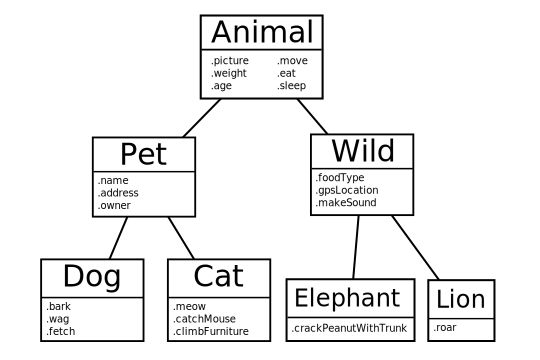
\includegraphics[scale=0.9]{fig-animal-class-chart.pdf}}}
\caption{Hierarquia de classes hipotética.}
\label{fig:animal-class-chart}
\end{figure}

OK---já basta desta explicação rapidinha sobre programação orientada a objetos. Vamos tentar alguns exemplos que você possa de fato rodar no SuperCollider. Rode uma linha após a outra e veja se você consegue identificar a mensagem, o objeto recebedor e o argumento (se houver). A estrutura básica é \texttt{Recebedor.mensagem(argumentos)}. Respostas ao final do livro.\endnote{Primeira linha: o Array \texttt{[1, 2, 3, "uau"]} é o objeto recebedor; \texttt{reverse} é a mensagem. Segunda linha: a String "alô" é o objeto recebedor; \texttt{dup} é a mensagem; \texttt{4} é o argumento para \texttt{dup}. Terceira linha: 3.1415 é o objeto recebedor; \texttt{round} é a mensagem; \texttt{0.1} é o argumento para \texttt{round}. Quarta linha: \texttt{100} é o objeto recebedor, \texttt{rand} é a mensagem. Última linha: \texttt{100.0} é o recebedor da mensagem \texttt{rand}, o resultado do qual é um número aleatório entre 0 e 100. Este número se torna o recebedor da mensagem \texttt{round} com o argumento \texttt{0.01}, assim o número aleatório é arredondado em duas casas decimais. Daí este resultado se torna o objeto recebedor da mensagem \texttt{dup} com o argumento \texttt{4}, que cria uma lista com quatro duplicatas daquele número.}

 
\begin{lstlisting}[style=SuperCollider-IDE, basicstyle=\scttfamily\footnotesize]
[1, 2, 3, "uau"].reverse;
"alô".dup(4); 
3.1415.round(0.1); // note que o primeiro ponto é a separação decimal de 3.1415 [N.T.: Atenção: o SC separa casas decimais com ponto! Vírgulas têm outros usos.]
100.rand; // rode esta linha diversas vezes;
// Encadear mensagens é divertido:
100.0.rand.round(0.01).dup(4);
\end{lstlisting}

\section{Receiver notation, functional notation}

There is more than one way of writing your expressions in SuperCollider. The one we just saw above is called \emph{receiver notation}: \texttt{100.rand}, where the dot connects the Object (\texttt{100}) to the message (\texttt{rand}). Alternatively, the exact same thing can also be written like this: \texttt{rand(100)}. This one is called \emph{functional notation}.

You can use either way of writing. Here's how this works when a message takes two or more arguments.

 
\begin{lstlisting}[style=SuperCollider-IDE, basicstyle=\scttfamily\footnotesize]
5.dup(20);  // receiver notation
dup(5, 20); // same thing in functional notation

3.1415.round(0.1); // receiver notation
round(3.1415, 0.1); // functional notation
\end{lstlisting}
 

In the examples above, you might read \texttt{dup(5, 20)} as ``duplicate the number 5 twenty times,'' and \texttt{round(3.1415, 0.1)} as ``round the number 3.1415 to one decimal case.'' Conversely, the receiver notation versions could be read as ``Number 5, duplicate yourself twenty times!'' (for \texttt{5.dup(20)}) and ``Number 3.1415, round yourself to one decimal case!'' (for \texttt{3.1415.round(0.1)}).

In short: \texttt{Receiver.message(argument)} is equivalent to \texttt{message(Receiver, argument)}.

Choosing one writing style over another is a matter of personal preference and convention. Sometimes one method can be clearer than the other. Whatever style you end up preferring (and it's fine to mix them), the important thing is to be consistent. One convention that is widespread among SuperCollider users is that classes (words that begin with uppercase letters) are almost always written as \texttt{Receiver.message(argument)}. For example, you will always see \texttt{SinOsc.ar(440)}, but you will almost never see \texttt{ar(SinOsc, 440)}, even though both are correct.

Exercise: rewrite the following statement using functional notation only:

\texttt{100.0.rand.round(0.01).dup(4);} 

Solution at the end.\endnote{Rewriting using functional notation only: \texttt{dup(round(rand(100.0), 0.01), 4);}}
\section{Aninhamento}
\label{sec:nesting}

A solução do último exercício levou você a aninhar coisas uma dentro da outra. David Cottle tem uma explicação excelente para aninhamento no The SuperCollider Book, então simplesmente o citaremos aqui.\footnote{Cottle, D. ``Beginner's Tutorial.'' The SuperCollider Book, MIT Press, 2011, pp. 8-9.}

\begin{quotation}
\textit{Para explicar melhor a ideia de aninhamento considere um exemplo hipotético no qual o SC vai preparar sua refeição. Para fazer isso você pode usar uma mensagem} \texttt{servir}. \textit{Os argumentos podem ser salada, prato principal e sobremesa. Mas apenas dizer} \texttt{servir(alface, peixe, banana)} \textit{talvez não produza o resultado que você quer. Então para ficar seguro você pode explicar estes argumentos, substituindo-os por uma mensagem aninhada e um argumento.}
\end{quotation}

\texttt{servir(misturar(alface, tomate, queijo), assar(peixe, 400, 20), bater(banana, sorvete))
}
\begin{quotation}
\textit{o SC então não apenas servirá alface peixe e banana, mas uma salada mista com alface, tomate e queijo; um peixe assado e um sundae de banana. Estes comandos internos podem ser ainda mais explicados, aninhando uma mensagem(arg) para cada ingrediente: alface, tomate, queijo e assim por diante. Cada mensagem interna produz um resultado que por sua vez é usado como argumento pela mensagem exterior.}
\end{quotation}

\begin{lstlisting}[style=SuperCollider-IDE, basicstyle=\scttfamily\footnotesize, label=code-dinner]
// Pseudo-código para fazer o jantar: 
servir(
	misturar(
		lavar(alface, água, 10),
		picar(tomate, pequendo),
		salpicar(escolher([gorgonzola, feta, gouda]))
	),
	assar(pegar(lagoa, anzol, vara), 400, 20),
	misturar(
		fatiar(descascar(banana), 20),
		cozinhar(misturar(leite, açúcar, amido), 200, 10)
	)
);
\end{lstlisting}

\begin{quotation}
\textit{Quando o aninhamento tem diversos níveis, podemos usar novas linhas e indentações para uma maior clareza. Algumas mensagens e argumentos estão à esquerda em uma linha, alguns estão distribuídos com um argumento por linha---o que quer seja mais claro. Cada nível de indentação deve indicar um nível de aninhamento. (Note que você pode ter qualquer quantidade de espaço em branco---novas linhas, tabulações e espaços---entre trechos de código.)}

[No exemplo do jantar,]\textit{ ao programa de refeições agora se pede para lavar a alface em água por 10 minutos e para picar o tomate em pequenos pedaços antes de misturá-los na travessa da salada e salpicá-los com queijo. Você também especificou onde pegar o peixe e disse para assá-lo a 400 graus por 20 minutos antes de servir e assim por diante.} 
\textit{Para "ler" este estilo de código, você começa da mensagem aninhada mais interna e vai seguindo para fora camada por camada. Aqui está um exemplo alinhado de maneira a mostrar como a mensagem mais interna é aninhada dentro das outras mensagens.}
\end{quotation}

%\lstinputlisting[style=SuperCollider-IDE, basicstyle=\scttfamily\footnotesize]{code-nesting.scd}

\begin{lstlisting}[style=SuperCollider-IDE, basicstyle=\scttfamily\footnotesize]
                exprand(1.0, 1000.0);
           dup({exprand(1.0, 1000.0)}, 100);
      sort(dup({exprand(1.0, 1000.0)}, 100));
round(sort(dup({exprand(1.0, 1000.0)}, 100)), 0.01);
\end{lstlisting}

O código abaixo é um outro exemplo de aninhamento. Responda às perguntas que se seguem. Você não precisa explicar o que os números estão fazendo---a tarefa é simplesmente idenftificar os argumetnos em cada camada de aninhamento. (Este exemplo e as questões do exercício também são emprestadas e ligeiramente modificadas do tutorial do Cottle.)

 
%\lstinputlisting[style=SuperCollider-IDE, basicstyle=\scttfamily\footnotesize, label=code-nested-music]{code-nested-music.scd}

\begin{lstlisting}[style=SuperCollider-IDE, basicstyle=\scttfamily\footnotesize]
// Aninhamento e indentação apropriada
(
{
	CombN.ar(
		SinOsc.ar(
			midicps(
				LFNoise1.ar(3, 24,
					LFSaw.ar([5, 5.123], 0, 3, 80)
				)
			),
			0, 0.4
		),
		1, 0.3, 2)
}.play;
)
\end{lstlisting}

\begin{enumerate}[a)]
\item Qual número é o segundo argumento para \texttt{LFNoise1.ar}?
\item Qual o primeiro argumento para \texttt{LFSaw.ar}?
\item Qual o terceiro argumento para \texttt{LFNoise1.ar}?
\item Quantos argumentos estão em \texttt{midicps}?
\item Qual o terceiro argumento para \texttt{SinOsc.ar}?
\item Qual o segundo e terceiro argumentos para \texttt{CombN.ar}?
\end{enumerate}

Confira as respostas ao final deste documento.\endnote{ Respostas: 
\begin{enumerate}[a)]
\item 24
\item $\left[5, 5.123\right]$ (tanto números quanto colchetes)
\item Toda a linha do \texttt{LFSaw}
\item Somente um
\item 0.4
\item 1 e 0.3
\end{enumerate}
 }

\medskip
 
\bigskip
\todo[inline, color=green!40]{ 
DICA: Se por qualquer motivo, seu código perdeu a indentação apropriada, simplesmente selecione tudo e vá para o menu Edit$\rightarrow$Autoindent Line or Region ("Autoindentar Linha ou Região") e isto será consertado.
}
\bigskip

\section{Enclosures}

There are four types of enclosures: \texttt{(parentheses)}, \texttt{[brackets]}, \texttt{\{braces\}}, and \texttt{"quotation marks"}.

Each one that you open will need to be closed at a later point. This is called ``balancing,'' that is, keeping properly matched pairs of enclosures throughout your code.

The SuperCollider IDE automatically indicates matching parentheses (also brackets and braces) when you close a pair---they show up in red. If you click on a parenthesis that lacks an opening/closing match, you will see a dark red selection telling you something is missing. Balancing is a quick way to select large sections of code for evaluation, deletion, or copy/paste operations. You can double click an opening or closing parenthesis (also brackets and braces) to select everything within.

\subsection{Quotation marks}

Quotation marks are used to enclose a sequence of characters (including spaces) as a single unit. These are called Strings. Single quotes create Symbols, which are slightly different than Strings. Symbols can also be created with a backslash immediately before the text. Thus \texttt{'greatSymbol'} and \texttt{\textbackslash greatSymbol} are equivalent.

\begin{lstlisting}[style=SuperCollider-IDE, basicstyle=\scttfamily\footnotesize]
"Here's a nice string";
'greatSymbol';
\end{lstlisting}

\subsection{Parentheses}

Parentheses can be used to:

\begin{itemize}
\item enclose argument lists: \texttt{rrand(0, 10);}
\item force precedence: \texttt{5 + (10 * 4);}
\item create code blocks (multiple lines of code to be evaluated together).
\end{itemize} 

\subsection{Brackets}

Square brackets define a collection of items, like \texttt{[1, 2, 3, 4, "hello"]}. These are normally called Arrays. An array can contain anything: numbers, strings, functions, patterns, etc. Arrays understand messages such as \texttt{reverse}, \texttt{scramble}, \texttt{mirror}, \texttt{choose}, to name a few. You can also perform mathematical operations on arrays.

\begin{lstlisting}[style=SuperCollider-IDE, basicstyle=\scttfamily\footnotesize]
[1, 2, 3, 4, "hello"].scramble;
[1, 2, 3, 4, "hello"].mirror;
[1, 2, 3, 4].reverse + 10;
// convert midi to frequency in Hz
[60, 62, 64, 65, 67, 69, 71].midicps.round(0.1);
\end{lstlisting}

More on Arrays coming soon in section \ref{sec:arrays}.

\subsection{Curly Braces}

Braces (or ``curly braces'') define functions. Functions encapsulate some kind of operation or task that will probably be used and reused multiple times, possibly returning different results each time. The example below is from the SuperCollider book.

\begin{lstlisting}[style=SuperCollider-IDE, basicstyle=\scttfamily\footnotesize]
exprand(1, 1000.0);
{exprand(1, 1000.0)};
\end{lstlisting}

David Cottle walks us through his example: \textit{``the first line picks a random number, which is displayed in the post window. The second prints a very different result: a function. What does the function do? It picks a random number. How can that difference affect code? Consider the lines below. The first chooses a random number and duplicates it. The second executes the random-number-picking function 5 times and collects the results in an array.''}\footnote{Cottle, D. ``Beginner's Tutorial.'' The SuperCollider Book, MIT Press, 2011, p. 13.}

\begin{lstlisting}[style=SuperCollider-IDE, basicstyle=\scttfamily\footnotesize]
rand(1000.0).dup(5);  // picks a number, duplicates it
{rand(1000.0)}.dup(5);  // duplicates the function of picking a number
{rand(1000.0)}.dup(5).round(0.1); // all of the above, then round
// essentially, this (which has a similar result)
[rand(1000.0), rand(1000.0), rand(1000.0), rand(1000.0), rand(1000.0)]
\end{lstlisting}
 

More about functions soon. For now, here's a summary of all possible enclosures:
\begin{description}
\item[Collections] \texttt{[list, of, items]}
\item[Functions] \texttt{\{ often multiple lines of code \}}
\item[Strings] \texttt{"words inside quotes"}
\item[Symbols] \texttt{'singlequotes'} or preceded by a \texttt{\textbackslash backslash}
\end{description}
\section{Condicionais: if/else e case}

Se estiver chovendo, saio com um guarda-chuva. Se estiver sol, saio com meus óculos escuros. Nosso dia-a-dia está repleto desse tipo de tomada de decisão. Em programação, estes são os momentos em que o seu código tem de testar alguma condição e realizar ações diferentes dependendo do resultado do teste (verdadeiro ou falso). Há muitos tipos de estruturas condicionais. Vamos dar uma olhada em dois casos simples: \emph{if/else} ("se/senão") e \emph{case} ("no caso de").

A sintaxe de um if/else no SC é: \texttt{if(condition, \{true action\}, \{false action\})}. A condição é um teste booleano, ou seja, precisa retornar um \texttt{true} ("verdadeiro") ou \texttt{false} ("falso"). Se o teste retorna verdadeiro, a primeira função é executada. Se não for verdadeiro, roda-se a segunda. Experimente:

\begin{lstlisting}[style=SuperCollider-IDE, basicstyle=\scttfamily\footnotesize]
// if / else 
if(100 > 50, { "muito verdadeiro".postln }, { "muito falso".postln });
\end{lstlisting}

A tabela abaixo, emprestada do The SuperCollider Book\footnote{Cottle, D. "Beginner's Tutorial." The SuperCollider Book, MIT Press, 2011, p. 33}, apresenta alguns operadores booleanos comuns que podem ser usados.
Note a distinção entre um sinal de igual simples (\texttt{x = 10}) e o sinal de igual duplo (\texttt{x == 10}). O simples significa "\textit{atribua 10 à variável x}," ao passo que o duplo significa "\textit{é x igual a 10?}" Digite e rode alguns exemplos da coluna de verdadeiro ou falso e você verá parecerem os resultados \texttt{true} ou  \texttt{false} aparecerem na Post window.
 
\begin{center}
\begin{tabular}{llll}
\hline 
\textbf{Símbolo} & \textbf{Significado} & \textbf{Exemplo verdadeiro} & \textbf{Exemplo falso} \\ 
\hline 
\texttt{==} & igual a? & \texttt{10 == 10} & \texttt{10 == 99} \\ 
\hline 
\texttt{!=} & diferente de? & \texttt{10 != 99} & \texttt{10 != 10} \\ 
\hline 
\texttt{>} & maior que? & \texttt{10 > 5} & \texttt{10 > 99} \\ 
\hline 
\texttt{<} & menor que? & \texttt{10 < 99} & \texttt{10 < 5} \\ 
\hline 
\texttt{>=} & maior ou igual a?  & \texttt{10 >= 10}, \texttt{10 >= 3} & \texttt{10 >= 99} \\ 
\hline 
\texttt{<=} & menor ou igual a? & \texttt{10 <= 99}, \texttt{10 <= 10} & \texttt{10 <= 9} \\ 
\hline 
\texttt{odd} & é ímpar? & \texttt{15.odd} & \texttt{16.odd} \\ 
\hline 
\texttt{even} & é par? & \texttt{22.even} & \texttt{21.even} \\ 
\hline 
\texttt{isInteger} & é um número inteiro? & \texttt{3.isInteger} & \texttt{3.1415.isInteger} \\ 
\hline 
\texttt{isFloat} & é um número decimal? & \texttt{3.1415.isFloat} & \texttt{3.isFloat} \\ 
\hline 
\texttt{and} & ambas as condições & \texttt{11.odd.and(12.even)} & \texttt{11.odd.and(13.even)} \\ 
\hline 
\texttt{or} & uma das condições & \texttt{or(1.odd, 1.even)} & \texttt{or(2.odd, 1.even)} \\ 
\hline 
\end{tabular} 
\end{center}
 

As últimas duas linhas (\texttt{and}, \texttt{or}) mostram como escrever as expressões mais longas tanto em notação de objeto recebedor quanto em notação funcional.

Outra estrutura útil é \texttt{case}. Ela funciona definindo pares de funções a serem executadas em ordem até que um dos testes retorne verdadeiro:

\texttt{case}

\texttt{\{teste1\} \{ação1\}}

\texttt{\{teste2\} \{ação2\}}

\texttt{\{teste3\} \{ação3\}}

\dots

\texttt{\{testeN\} \{açãoN\}};

A expressão dentro de cada teste tem de retornar ou \texttt{true} ou \texttt{false}. Se o teste1 retorna falso, o programa ignora a ação1 e segue para o teste2. Se teste2 for um falso de novo, ação2 também é ignorada e seguimos para o teste3. Se este for verdadeiro, então a ação3 é executada e o \texttt{case} se encerra ali (mais nenhum teste ou ação é executado). Note que não há vírgulas entre as funções. Simplesmente use um ponto-e-vírgula no fim para marcar o final do enunciado \texttt{case}.

 
\begin{lstlisting}[style=SuperCollider-IDE, basicstyle=\scttfamily\footnotesize]
// case
(
~num = -2;

case
{~num == 0} {"UAU".postln}
{~num == 1} {"UM!".postln}
{~num < 0} {"número negativo!".postln}
{true} {"em último caso".postln};
)
\end{lstlisting}
 
Tente modificar o código acima para obter todos os resultados possíveis. Perceba o truque útil (e opcional) na última linha de \texttt{case} no exemplo acima: como \texttt{true} sempre retorna verdadeiro, pode-se definir uma ação para acontecer "em último caso" que vai sempre ocorrer, mesmo no caso de todas as condições anteriores serem falsas.

Para saber mais, verifique o arquivo de ajuda de Control Structures ("Estruturas de Controle").

\section{Funções}
\label{sec:functions}

Quando você se pegar repetindo a mesma tarefa diversas vezes, talvez seja um bom momento para criar uma função reutilizável. Uma função, como você aprendeu na seção de Fechamentos, é algo escrito entre chaves. David Touretzky introduz a ideia de função da seguinte forma: "pense na função como uma caixa através da qual os dados passam. Essa função opera sobre os dados de alguma forma e o resultado é o que passa para fora." \footnote{Touretzky, David. COMMON LISP: A Gentle Introduction to Symbolic Computation. The Benjamin/Cummings Publishing Company, Inc, 1990, p. 1. Este é o livro que inspirou o título original em inglês deste tutorial.}

\begin{figure}[h]
\centerline{\framebox{
	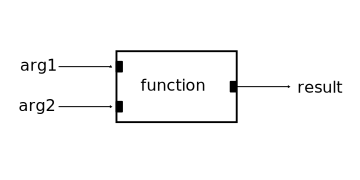
\includegraphics[scale=0.9]{fig-function-box.pdf}}}
\caption{Ideia geral de uma função.}
\label{fig:function-box}
\end{figure}

A primeira linha no exemplo abaixo define a função, atribuindo-a à variável \texttt{f}. A segunda linha coloca a função para trabalhar.

 
\begin{lstlisting}[style=SuperCollider-IDE, basicstyle=\scttfamily\footnotesize]
f = { 2 + 2 }; // define a função
f.value; // põe a função para trabalhar
\end{lstlisting}
 
A função acima não é lá muito útil, pois sabe fazer uma coisa só (somar 2 e 2). Normalmente a gente quer definir funções que possam dar diferentes resultados dependendo dos argumentos de entrada fornecidos. Nós usamos a palavra-chave \texttt{arg} para especificar as entradas que uma função vai aceitar. O exemplo abaixo é mais parecido com o desenho da figura \ref{fig:function-box}.
 
\begin{lstlisting}[style=SuperCollider-IDE, basicstyle=\scttfamily\footnotesize]
f = {arg a, b; ["a mais b", a+b, "a vezes b", a*b].postln}; // define função
f.value(3, 7); // forneça dois números quaisquer como argumentos para a função
f.value(10, 14);

// Compare:
~aleaTonto = rrand(0, 10); // não é uma função
~aleaTonto.value; // execute diversas vezes
~aleaTonto2 = {rrand(0, 10)}; // é uma função
~aleaTonto2.value; // execute diversas vezes
\end{lstlisting}
 
Como um último exemplo, aqui está uma função muito útil.
 
\begin{lstlisting}[style=SuperCollider-IDE, basicstyle=\scttfamily\footnotesize]
// Use esta função para decidir como passar seus dias de verão

(
~oQueFazer = { 
var hoje, nomeDoDia, acoes;
	hoje = Date.getDate.dayOfWeek;
	nomeDoDia = 
	case
	{hoje==0} {"Domingo"}
	{hoje==1} {"Segunda"}
	{hoje==2} {"Terça"}
	{hoje==3} {"Quarta"}
	{hoje==4} {"Quinta"}
	{hoje==5} {"Sexta"}
	{hoje==6} {"Sábado"};
	acoes = ["jogar bumerangue", "queda de braço", "subir escadas", "jogar xadrez", "basquete subaquático", "arremesso de ervilhas", "longa soneca"];
	"Ah, " ++ nomeDoDia ++ "...! " ++ "Que ótimo dia para " ++ acoes.choose;
};
)

// Execute pela manhã
~oQueFazer.value;
\end{lstlisting}

\bigskip
\todo[inline, color=green!40]{ DICA: Outra notação comum para declarar argumentos no início de uma Função é: \texttt{f = \{|a, b| a + b\}}. Isso é equivalente a \texttt{f = \{arg a, b; a + b\}}} 


\section{Divirta-se com Arrays}
\label{sec:arrays}

Arrays [N.T.: em computação, o termo "array" pode ser traduzido como "vetor", mas é comum mantê-lo no original] são o tipo mais comum de coleção no SuperCollider. Toda vez que você escreve uma coleção de itens entre colchetes, como \texttt{[0, 1, 2]}, cria uma instância da classe \texttt{Array}. Frequentemente, você se verá manipulando arrays de diversas formas. Aqui está uma pequena seleção de métodos interessantes que arrays entendem:

 
\begin{lstlisting}[style=SuperCollider-IDE, basicstyle=\scttfamily\footnotesize]
// Criar uma array
a = [10, 11, 12, 13, 14, 15, 16, 17];

a.reverse; // inverter
a.scramble; // embaralhar
a.choose; // escolher um elemento ao acaso
a.size; // retorna o tamanho da array
a.at(0); // recupera um item na posição especificada
a[0]; // o mesmo que acima
a.wrapAt(9); // recupera item na posição especificada, relendo do início se > a.size
["wow", 99] ++ a; // concatena duas arrays em uma nova
a ++ \oi; // um Símbolo é entendido como um único caracter
a ++ 'oi'; // o mesmo que acima
a ++ "oi"; // uma cadeia ("String") é entendida como uma coleção de caracteres
a.add(44); // cria uma nova array adicionando o novo elemento ao final
a.insert(5, "uau"); // insere "uau" na posição 5, empurra itens seguintes para a frente (retorna uma nova array)
a; // rode isso e veja que nenhuma das operações acima mudou a array original
a.put(2, "oops"); // colocar "oops" no índice 2 (destrutivo; volte a rodar a linha acima para verificar)
a.permute(3); // permutar: item na posição 3 vai para a posição zero, e vice-versa
a.mirror; // faz um palíndromo
a.powerset; // retorna todas as possíveis combinações dos elementos da array
\end{lstlisting}
 

Você pode fazer contas com arrays:

 
\begin{lstlisting}[style=SuperCollider-IDE, basicstyle=\scttfamily\footnotesize]
[1, 2, 3, 4, 5] + 10;
[1, 2, 3, 4, 5] * 10;
([1, 2, 3, 4, 5] / 7).round(0.01); // note o uso de parênteses para precedência
x = 11; y = 12; // experimente algumas variáveis
[x, y, 9] * 100;
// mas garanta que você só faça contas com números de verdade
[1, 2, 3, 4, "oops", 11] + 10; // resultado estranho
\end{lstlisting}
 

\subsection{Creating new Arrays}

Aqui há algumas maneiras de usar a classe \texttt{Array} para criar novas coleções:

\begin{lstlisting}[style=SuperCollider-IDE, basicstyle=\scttfamily\footnotesize]
// Progressão aritmética (definindo tamanho, início e passo da progressão)
Array.series(size: 6, start: 10, step: 3);
// Progressão geométrica (definindo tamanho, início e razão da progressão)
Array.geom(size: 10, start: 1, grow: 2);
// Compare as duas:
Array.series(7, 100, -10); // 7 itens; começando em 100, passo de -10
Array.geom(7, 100, 0.9); // 7 itens; começando em 100; multiplicar por 0.9 a cada vez
// Conheça o método .fill
Array.fill(10, "igual");
// Compare:
Array.fill(10, rrand(1, 10)); 
Array.fill(10, {rrand(1, 10)}); // a função é reexecutada 10 vezes
// A função definida como segundo arg do método .fill pode receber um contador como argumento padrão.
// O nome do argumento pode ser o que você quiser.
Array.fill(10, {arg contador; contador * 10});
// Por exemplo, gerando uma lista de frequências harmônicas:
Array.fill(10, {arg uau; uau+1 * 440}); 
// O método .newClear
a = Array.newClear(7); // cria uma array vazia do tamanho desejado
a[3] = "uau"; // mesmo que a.put(3, "uau")
\end{lstlisting}


\subsection{Aquele ponto de exclamação esquisito}

É só uma questão de tempo até que você veja algo como \texttt{30!4} no código de alguém. Essa notação abreviada simplesmente cria uma array contendo o mesmo item um determinado número de vezes:

 
\begin{lstlisting}[style=SuperCollider-IDE, basicstyle=\scttfamily\footnotesize]
// Notação abreviada:
30!4;
"alô" ! 10;
// Dá o mesmo resultado que o seguinte:
30.dup(4);
"alô".dup(10);
// ou
Array.fill(4, 30);
Array.fill(10, "alô");
\end{lstlisting}
 

\subsection{Os dois pontos entre parênteses}

Aqui está mais uma sintaxe abreviada muito usada para criar arrays.

 
\begin{lstlisting}[style=SuperCollider-IDE, basicstyle=\scttfamily\footnotesize]
// Que diabo é isso?
(50..79);
// É um atalho para gerar uma array com uma progressão numérica aritmética.
// O atalho acima tem o mesmo resultado que:
series(50, 51, 79);
// ou
Array.series(30, 50, 1);
// Para um passo (razão) diferente de 1, você pode fazer o seguinte:
(50, 53 .. 79); // de 3 em 3
// Mesmo resultado que:
series(50, 53, 79);
Array.series(10, 50, 3);
\end{lstlisting}

Note que cada comando implica um jeito de pensar ligeiramente diferente. O \texttt{(50..79)} permite que você pense assim: "\emph{me dê uma array de 50 a 79}." Você não precisa necessariamente pensar a quantidade de itens que a lista vai conter. Por outro lado, \texttt{Array.series} permite pensar: "\emph{me dê uma array com 30 itens no total, começando a partir do 50}." Você não precisa necessariamente pensar qual será o último número da série.

Também note que o atalho usa parênteses, não colchetes. A array resultante, naturalmente, virá entre colchetes.
\subsection{Como "fazer" um Array}

Muitas vezes você vai precisar realizar alguma operação com cada um dos itens de uma coleção. Você pode usar o método \texttt{do} ("faça") para isso:


\begin{lstlisting}[style=SuperCollider-IDE, basicstyle=\scttfamily\footnotesize]
~minhasFreqs = Array.fill(10, {rrand(440, 880)});

//Agora vamos fazer uma ação simples com cada um dos itens da lista:
~minhasFreqs.do({arg item, contador; ("Item " ++ contador ++ " é " ++ item ++ " Hz. A nota MIDI mais próxima é " ++ item.cpsmidi.round).postln});

// Se você não precisa do contador, use apenas um argumento:
~minhasFreqs.do({arg item; item.squared.postln});

// Claro que algo simples como o exemplo anterior poderia ser feito assim:
~minhasFreqs.squared;
\end{lstlisting}
 

Em resumo: quando você processa uma array com "do", você fornece uma função. A mensagem \texttt{"do"} vai cuidar de executar a função uma vez para cada item constante da array. A função pode receber dois argumentos por definição: o item da vez propriamente dito, e um contador que vai registrando o número de iterações já realizadas. Os nomes destes argumentos podem ser o que você quiser, mas estarão sempre nesta ordem: item, contador.

Veja também o método \texttt{collect}, que é muito similar ao \texttt{do}, mas retorna uma nova coleção com todos os resultados intermediários.

\section{Getting Help}

Learn how to make good use of the Help files. Often you will find useful examples at the bottom of each Help page. Be sure to scroll down to check them out, even (or specially) if you don't fully understand the text explanations at first. You can run the examples directly from the Help browser, or you can copy and paste the code onto a new window to play around with it. 

Select any valid class or method in your SuperCollider code (double-clicking the word will select it), and hit [ctrl+D] to open the corresponding Help file. If you select a class name (for example, \texttt{MouseX}), you will be directed to the class Help file. If you select a method, you will be directed to a list of classes that understand that method (for example, ask for help on the method \texttt{scramble}).\footnote{Attention: SuperCollider will display in blue any word that starts with a Capital letter. This means that the color blue \emph{does not guarantee} that the word is typo-free: for example, if you type Sinosc (with wrong lowercase "o"), it will still show up in blue.}

Other ways to explore the Help files in the SuperCollider IDE are the ``Browse'' and ``Search'' links. Use Browse to navigate the files by categories, and Search to look for words in all Help files. Important note about the Help Browser in the SuperCollider IDE:
\begin{itemize}
\item Use the top-right field (where it says ``Find...'') to look for specific words \emph{within the currently open Help file} (like you would do a ``find'' on a website);
\item Use the ``Search'' link (to the right of ``Browse'') to search text \emph{across all Help files}.
\end{itemize}

When you first open parentheses to add arguments to a given method, SC displays a little ``tooltip help'' to show you what the expected arguments are. For example, type the beginning of line that you see in figure \ref{fig:tooltip}. Right after opening the first parenthesis, you see the tooltip showing that the arguments to a \texttt{SinOsc.ar} are \texttt{freq}, \texttt{phase}, \texttt{mul}, and \texttt{add}. It also shows us what the default values are. This is exactly the same information you would get from the \texttt{SinOsc} Help file. If the tooltip has disappeared, you can bring it back with [ctrl+Shift+Space].

\begin{figure}[h]
\centerline{\framebox{
	\includegraphics[scale=0.3]{fig-help-tooltip-crop.png}}}
\caption{Helpful info is displayed as you type.}
\label{fig:tooltip}
\end{figure}

Another shortcut: if you would like to explicitly name your arguments (like \texttt{SinOsc.ar(freq: 890)}), try hitting the tab key right after opening the parentheses. SC will autocomplete the correct argument name for you, in order, as you type (hit tab after the comma for subsequent argument names).

\bigskip
\todo[inline, color=green!40]{ 
TIP: Create a folder with your own ``personalized help files.'' Whenever you figure out some new trick or learn a new object, write a simple example with explanations in your own words, and save it for the future. It may come in handy a month or a year from now. 
}
\bigskip

The exact same Help files can also be found online at \url{http://doc.sccode.org/}.
% PART IV
\newpage
\part{SÍNTESE E PROCESSAMENTO SONORO}
Você já aprendeu bastante coisas sobre o SuperCollider. Nas seções anteriores, este tutorial apresentou para você detalhes minuciosos sobre a própria linguagem, de variáveis a fechamentos e muito mais. Você também aprendeu como criar \texttt{Pbind}s interessantes, usando vários membros da família Pattern.

Esta parte do tutorial vai (finalmente!) apresentar síntese e processamento sonoros com o SuperCollider. Começaremos com o tópico das Unit Generators ("Unidades Geradoras" ou "Geradores Unitários", que daqui em diante chamaremos UGens). \footnote{A maioria dos tutoriais começa diretamente com as UGens; nesta introdução ao SC, no entanto, escolhemos primeiro enfatizar a família Pattern (\texttt{Pbind} e sua turma) para uma abordagem pedagógica diferente.}

\section{UGens}

Você já viu algumas Unidades Geradoras (UGens) em ação nas seções \ref{sec:first-sine} e \ref{sec:nesting}. O que é uma UGen? Uma unidade geradora é um objeto que gera sinais sonoros ou sinais de controle. Estes sinais são sempre calculados no servidor. Há muitas classes de unidades geradoras, todas elas derivando da classe UGen. \texttt{SinOsc} e \texttt{LFNoise0} são exemplos de UGens. Para mais detalhes, veja os arquivos de Ajuda chamados "Unit Generators and Synths" e "Tour of UGens". 

Quando você tocou seus Pbinds uns capítulos atrás, o som padrão era sempre o mesmo: um sintetizador simples semelhante a um piano. Este sintetizador é feito de uma combinação de unidades geradoras.\footnote{Como você usou \texttt{Pbind}s até aqui para fazer som no SuperCollider, pode ser tentador pensar: \textit{"Entendi, então o \texttt{Pbind} é uma Unidade Geradora!"} Não é o caso. \texttt{Pbind} não é uma Unidade Geradora---ele é apenas uma receita para fazer eventos musicais (partitura). \textit{"Então o \texttt{EventStreamPlayer}, a coisa que aparece quando eu chamo \texttt{play} em um \texttt{Pbind}, ISSO deve ser uma UGen!"} A resposta ainda é não. O \texttt{EventStreamPlayer} é apenas o tocador, como um pianista, e o pianista não gera som. Continuando com esta comparação didática, o \emph{instrumento piano} é a coisa que realmente vibra e produz som. Está é uma analogia mais adequada para a UGen: não é a partitura, não é o tocador: é o instrumento. Quando você fez música com \texttt{Pbind}s antes, o SC criava um \texttt{EventStreamPlayer} para tocar sua partitura com seu sintetizador de piano embutido. Você não tinha de se preocupar em criar o piano ou algo assim---o SuperCollider fez todo o trabalho nos bastidores para você. Aquele sintetizador de piano escondido é feito de uma combinação de algumas Unidades Geradoras.} Você aprenderá como combinar unidades geradoras para criar todo tipo de instrumentos com sons sintéticos e processados. O próximo exemplo parte da nossa primeira senoide para criar um instrumento eletrônico que você pode tocar ao vivo com o mouse.

\subsection{Controle do Mouse: Theremin instantâneo}

Aqui está um sintetizador simples que você pode tocar em tempo real. É uma simulação do Theremin, um dos mais antigos instrumentos eletrônicos:

\begin{lstlisting}[style=SuperCollider-IDE, basicstyle=\scttfamily\footnotesize]
{SinOsc.ar(freq: MouseX.kr(300, 2500), mul: MouseY.kr(0, 1))}.play;
\end{lstlisting}

Se você não sabe o que é um Theremim, por favor pare tudo que está fazendo e procure por "Clara Rockmore Theremin" no YouTube. Depois volte aqui e tente tocar "O Cisne" com o seu Theremin de SuperCollider.

\texttt{SinOsc}, \texttt{MouseX} e \texttt{MouseY} são UGens. \texttt{SinOsc} está gerando o som da onda senoidal. Os outros dois estão captando o movimento do seu cursor na tela (X para o movimento horizontal e Y para o movimento vertical) e usando os números para alimentar os valores de frequência e amplitude da senoide. Bem simples, mas já bem divertido!

\subsection{Dente-de-serra e onda quadrada; gráfico e osciloscópio}

O Theremin acima usou um oscilador senoidal. Há outras formas de onda que você pode usar para fazer som. Rode as linhas abaixo---elas usam o conveniente método \texttt{plot} ("gráfico")---para olhar a forma do \texttt{SinOsc} e compará-lo com \texttt{Saw} e \texttt{Pulse}. As linhas abaixo não produzem som---elas apenas permitem que você visualize um trecho da forma de onda.

\begin{lstlisting}[style=SuperCollider-IDE, basicstyle=\scttfamily\footnotesize]
{ SinOsc.ar }.plot; // onda senoidal
{ Saw.ar }.plot; // onda dente-de-serra
{ Pulse.ar }.plot; // onda quadrada
\end{lstlisting}

Agora reescreva sua linha de Theremin, substituindo \texttt{SinOsc} por \texttt{Saw}, depois por \texttt{Pulse}. Escute como eles soam diferente. Finalmente, experimente \texttt{.scope} em vez de \texttt{.play} no seu código de Theremin e você poderá ver uma representação da forma de onda em tempo real (abrirá uma janela "Stethoscope", que na realidade é um osciloscópio).

\section{Audio rate, control rate}

É bastante fácil identificar uma UGen em um código de SuperCollider: elas são quase sempre seguidas pelas mensagens \texttt{.ar} ou \texttt{.kr}. Estas letras querem dizer Audio Rate ("taxa de áudio") e Control Rate ("taxa de controle"). Vamos ver o que isso significa.

Do arquivo de ajuda "Unit Generators and Synths" ("Unidades geradoras e Sintetizadores"): 

\begin{quotation}
Uma unidade geradora é criada ao se enviar uma mensagem \texttt{ar} ou \texttt{kr} para um objeto da classe da respectiva unidade geradora. A mensagem \texttt{ar} cria uma UGen que é executada na velocidade da taxa de áudio. A mensagem \texttt{kr} cria uma UGen executada na velocidade da taxa de controle. UGens de controle são usados para sinais de controle de baixa frequência ou que mudam lentamente. UGens de controle produzem uma única amostra por ciclo de controle e, por isso, utilizam menos poder de processamento que UGens de áudio. \footnote{\url{http://doc.sccode.org/Guides/UGens-and-Synths.html}}
\end{quotation}

Em outras palavras: quando você escreve \texttt{SinOsc.ar}, você está mandando a mensagem "taxa de áudio" para a UGen \texttt{SinOsc} UGen. Assumindo que seu computador esteja rodando na taxa de amostragem comum de 44100 Hz, este oscilador senoidal vai gerar 44100 amostras por segundo para serem enviadas ao alto-falante. Então escutamos uma onda senoidal.

Reflita por um momento sobre o que você acabou de ler: quando você manda a mensagem \texttt{ar} para uma UGen, você esta pedindo que que ela gere \emph{quarenta e quatro mil e cem} números por segundo. Uma verdadeira enxurrada de números. Você escreve \texttt{\{SinOsc.ar\}.play} na linguagem e a linguagem comunica seu pedido ao servidor. O verdadeiro trabalho de gerar todas estas amostras é feito pelo servidor, o "motor sonoro" do SuperCollider.

Agora, quando você usa \texttt{kr} em vez de \texttt{ar}, o trabalho tambem é feito pelo servidor, mas há algumas diferenças:
\begin{enumerate}
\item A quantidade de números gerados por segundo com \texttt{.kr} é muito menor. \texttt{\{SinOsc.ar\}.play} gera 44100 números por segundo, enquanto \texttt{\{SinOsc.kr\}.play} produz perto de 700 números por segundo (se você tiver curiosidade, a quantidade exata é 44100 / 64, sendo que 64 é o chamado "período de controle".)
\item O sinal gerado com \texttt{kr} não vai para os alto-falantes. Em vez disso, é normalmente utilizado para controlar parâmetros de outros sinais---por exemplo, o \texttt{MouseX.kr} no seu theremim estava controlando a frequência de um \texttt{SinOsc}.

\end{enumerate} 

OK, então UGens são geradores de números incrivelmente velozes. Alguns destes números se tornam sinais sonoros; outros se tornam sinais de controle. Até aí, tudo bem. Mas que números são estes, afinal de contas? Grandes? Pequenos? Positivos? Negativos? Na verdade, são números bem pequenos, muitas vezes entre -1 e +1. Às vezes somente entre 0 e 1. Todas as UGens podem ser divididas em duas categorias, de acordo com a abrangência dos números que elas geram: UGens unipolares e UGens bipolares.

\begin{description}
\item[UGens unipolares] geram números entre 0 e 1.
\item[UGens bipolares] geram números entre -1 e +1.

\end{description}

\subsection{O método \texttt{poll}}

Vale a pena examinar a saída de algumas UGens para esclarecer isso. Não é uma boa ideia pedir pro SuperCollider imprimir milhares de números por segundo na Post window, mas podemos pedir que ele imprima algumas dezenas deles, só para termos uma ideia. Digite e rode as seguintes linhas, uma de cada vez (confirme que seu servidor esteja rodando), e observe a Post window: 

\begin{lstlisting}[style=SuperCollider-IDE, basicstyle=\scttfamily\footnotesize]
// apenas observe a Post window (não vai fazer som)
{SinOsc.kr(1).poll}.play;
// pressione ctrl+ponto, daí rode a próxima linha:
{LFPulse.kr(1).poll}.play;
\end{lstlisting}

Os exemplos não produzem som algum porque estamos usando \texttt{kr}---o resultado é um sinal de controle, então nada é enviado para os alto-falantes. O objetivo aqui é apenas observar a saída típica de algumas UGens. A mensagem \texttt{poll} pega 10 números por segundo da saída do \texttt{SinOsc} e as imprime na Post window. O argumento 1 é a frequência da senoide, o que quer dizer que a onda senoidal vai demorar um segundo para completar um ciclo inteiro. Baseado no que você observou, o \texttt{SinOsc} é unipolar ou bipolar? E o \texttt{LFPulse}?\endnote{\texttt{SinOsc} é bipolar porque produz números entre 1- e +1. \texttt{LFPulse} é unipolar porque o âmbito de saída é 0-1 (repare que no caso do \texttt{LFPulse} em particular, somente "zeros" e "uns" são gerados, sem nenhum número intermediário)}

Abaixe todo o volume antes de rodar a próxima linha, depois aumente-o devagar. Você vai ouvir uns cliques suaves.

\begin{lstlisting}[style=SuperCollider-IDE, basicstyle=\scttfamily\footnotesize]
{LFNoise0.ar(1).poll}.play;
\end{lstlisting}

Como mandamos uma mensagem \texttt{ar} para esta Ugen, ela está enviando 44100 amostras por segundo para a sua placa de som---é um sinal de áudio. \texttt{LFNoise0} é um gerador de ruído de baixa frequência ("Low Frequency Noise"). Cada amostra é um número aleatoriamente escolhido entre -1 e +1 (então é uma UGen bipolar). Com \texttt{poll} você está vendo somente dez deles por segundo. \texttt{LFNoise0.ar(1)} escolhe um novo número randômico a cada segundo. Tudo isto é feito pelo servidor.

Pare os clicks com [ctrl+.] e experimente mudar a frequência de \texttt{LFNoise0}. Tente números como 3, 5, 10 e depois mais altos. Observe os números produzidos e ouça os resultados.

\section{UGen arguments}

Most of the time you will want to specify arguments to the UGens you are using. You have already seen that: when you write \texttt{\{SinOsc.ar(440)\}.play}, the number \texttt{440} is an argument to the \texttt{SinOsc.ar}; it specifies the frequency that you will hear. You can be explicit about naming the arguments, like this: \texttt{\{SinOsc.ar(freq: 440, mul: 0.5)\}.play}. The argument names are \texttt{freq} and \texttt{mul} (note the colon immediately after the words in the code). The \texttt{mul} stands for ``multiplier'', and is essentially the amplitude of the waveform. If you don't specify \texttt{mul}, SuperCollider uses the default value of 1 (maximum amplitude). Using a \texttt{mul: 0.5} means multiplying the waveform by half, in other words, it will play at half of the maximum amplitude.

In your theremin code, the \texttt{SinOsc} arguments \texttt{freq} and \texttt{mul} were explicitly named. You may recall that  \texttt{MouseX.kr(300, 2500)} was used to control the frequency of the theremin. \texttt{MouseX.kr} takes two arguments: a low and a high boundary for its output range. That's what the numbers 300 and 2500 were doing there. Same thing for the \texttt{MouseY.kr(0, 1)} controlling amplitude. Those arguments inside the mouse UGens were not explicitly named, but they could be.

How do you find out what arguments a UGen will accept? Simply go to the corresponding Help file: double click the UGen name to select it, and hit [ctrl+D] to open the Documentation page. Do that now for, say, MouseX. After the Description section you see the Class Methods section. Right there, it says that the arguments of the \texttt{kr} method are minval, maxval, warp, and lag. From the same page you can learn what each of them does.

Whenever you don't provide an argument, SC will use the default values that you see in the Help file. If you don't name the arguments explicitly, you have to provide them in the exact order shown in the Help file. If you do name them explicitly, you can put them in any order, and even skip some in the middle. Naming arguments explicitly is also a good learning tool, as it helps you to better understand your code. An example is given below.

\begin{lstlisting}[style=SuperCollider-IDE, basicstyle=\scttfamily\footnotesize]
// minval and maxval provided in order, no keywords
{MouseX.kr(300, 2500).poll}.play;
// minval, maxval and lag provided, skipped warp
{MouseX.kr(minval: 300, maxval: 2500, lag: 10).poll}.play;
\end{lstlisting}
\section{Redimensionando âmbitos (“ranges”)}

A verdadeira diversão começa quando você usa algumas UGens para controlar os parâmetros de outras UGens. O exemplo do theremin fez exatamente isto. Agora você tem todas as ferramentas para entender exatamente o que está acontecendo em um dos exemplos da seção \ref{sec:first-sine}. As três últimas linhas do exemplo demonstram passo a passo como o \texttt{LFNoise0} é usado para controlar a frequência:

\begin{lstlisting}[style=SuperCollider-IDE, basicstyle=\scttfamily\footnotesize]
{SinOsc.ar(freq: LFNoise0.kr(10).range(500, 1500), mul: 0.1)}.play;

// Separando em partes:
{LFNoise0.kr(1).poll}.play; // veja um simples LFNoise0 em ação
{LFNoise0.kr(1).range(500, 1500).poll}.play; // agora com .range
{LFNoise0.kr(10).range(500, 1500).poll}.play; // agora mais rápido
\end{lstlisting}

\subsection{Redimensione com o método \texttt{range}}
O método  \texttt{range} simplesmente redimensiona a saída de uma UGen. Lembre-se, \texttt{LFNoise0} produz números entre -1 e +1 (é uma UGen bipolar). Estes números brutos não seriam muito úteis para controlar frequência (precisamos de números perceptíveis na escala de audição humana). O \texttt{.range} pega esta saída entre -1 e +1 e a redimensiona entre qualquer valor mínimo e máximo que você fornecer como argumentos (neste caso, 500 e 1500). O número 10, que é o argumento para \texttt{LFNoise0.kr}, especifica a frequência da UGen: quantas vezes por segundos ele escolhe um novo número aleatório.

Resumindo: para usar a UGen para controlar algum parâmetro de outra UGen, primeiro você tem que saber qual o âmbito numérico que você quer. Os números serão frequências? Você os quer entre, digamos, 10 e 1000? Ou são amplitudes? Talvez você queira que as amplitudes estejam entre 0.1 (suave) e 0.5 (metade do máximo)? Ou você está tentando controlar o número de harmônicos? Você quer que ele esteja entre 5 e 19?

Uma vez que você sabe o âmbito que você precisa, use o método \texttt{.range} para fazer com que a UGen controladora faça a coisa certa.

Exercício: escreva uma linha de código simples que toca uma onda senoidal, cuja frequência é controlada por um \texttt{LFPulse.kr} (forneça agumentos apropriados para ele). Então, use o método \texttt{.range} para redimensionar a saída do \texttt{LFPulse} em algo que você queira escutar. 

\subsection{Redimensionando com \texttt{mul} e \texttt{add}}

Agora você sabe redimensionar a saída de UGens no servidor usando o método \texttt{.range}. A mesma coisa pode ser obtida em um nível mais fundamental usando os argumentos \texttt{mul} e \texttt{add}, que quase todos os UGens têm. O código abaixo mostra a equivalência entre as abordagens com \texttt{range} e de \texttt{mul/add}, ambos com uma UGen bipolar e uma UGen unipolar.

\begin{lstlisting}[style=SuperCollider-IDE, basicstyle=\scttfamily\footnotesize]
// Isso:
{SinOsc.kr(1).range(100, 200).poll}.play;
// …é o mesmo que isso:
{SinOsc.kr(1, mul: 50, add: 150).poll}.play;

// Isso:
{LFPulse.kr(1).range(100, 200).poll}.play;
// …é o mesmo que isso:
{LFPulse.kr(1, mul: 50, add: 100).poll}.play;
\end{lstlisting}

A figura \ref{fig:mul-add-scale} ajuda a visualizar como \texttt{mul} e \texttt{add} trabalham redimensionando as saídas de UGens (um \texttt{SinOsc} é usado como demonstração).

\begin{figure}[h!]
\centerline{\framebox{
	\includegraphics[scale=0.6]{fig-mul-add-scale.pdf}}}
\caption{Redimensionando âmbitos de UGens com mul e add}
\label{fig:mul-add-scale}
\end{figure}

\subsection{\texttt{linlin} e seus amigos}

Para qualquer outro redimensionamento arbitrário de âmbitos, você pode usar os práticos métodos \texttt{linlin}, \texttt{linexp}, \texttt{explin} e \texttt{expexp}. Os nomes nos métodos dão uma dica do que eles fazem: converter um âmbito linear em outro âmbito linear (\texttt{linlin}), linear para exponencial (\texttt{linexp}), etc.

\begin{lstlisting}[style=SuperCollider-IDE, basicstyle=\scttfamily\footnotesize]
// Um punhado de números
a = [1, 2, 3, 4, 5, 6, 7];
// Redimensione para 0-127, linear para linear
a.linlin(1, 7, 0, 127).round(1);
// Redimensione para 0-127, linear para exponencial
a.linexp(1, 7, 0.01, 127).round(1); // não use zero para um âmbito exponencial
\end{lstlisting}

Para uma revisão acerca de linear e exponencial, procure online a diferença entre progressões aritméticas e geométricas. Brevemente, sequências lineares (aritméticas) são como "1, 2, 3, 4, 5, 6" or "3, 6, 9, 12, 15", etc; e sequências exponenciais (geométricas) são como "1, 2, 4, 8, 16, 32" or "3, 9, 27, 81, 243", etc.




\section{Parando sintetizadores individualmente}

Eis um jeito bastante comum de iniciar diversos sintetizadores e ser capaz de interrompê-los separadamente. O exemplo é autoexplicativo:

\begin{lstlisting}[style=SuperCollider-IDE, basicstyle=\scttfamily\footnotesize]
// Rode uma linha de cada vez (não pare o som entre elas):
a = { Saw.ar(LFNoise2.kr(8).range(1000, 2000), mul: 0.2) }.play;
b = { Saw.ar(LFNoise2.kr(7).range(100, 1000), mul: 0.2) }.play;
c = { Saw.ar(LFNoise0.kr(15).range(2000, 3000), mul: 0.1) }.play;
// Pare os sintetizadores individualmente:
a.free;
b.free;
c.free; 	
\end{lstlisting}

\section{A mensagem \texttt{set}}

Assim como com qualquer função (reveja a seção \ref{sec:functions}), argumentos especificados no início da sua função de sintetizador ficam acessíveis ao usuário. Isso permite que você modifique parâmetros em tempo real (enquanto o sintetizador está rodando). A mensagem \texttt{set} ("definir") é usada para este fim. Exemplo simples:

\begin{lstlisting}[style=SuperCollider-IDE, basicstyle=\scttfamily\footnotesize]
x = {arg freq = 440, amp = 0.1; SinOsc.ar(freq, 0, amp)}.play;
x.set(\freq, 778);
x.set(\amp, 0.5);
x.set(\freq, 920, \amp, 0.2);
x.free;
\end{lstlisting}

É um bom hábito fornecer valores pré-definidos (como 440 e 0.1 acima), de outra forma o sintetizador não vai tocar até que você defina um valor apropriado para os parâmetros 'vazios'.

\section{Canais de Áudio}
\label{sec:audiobus}

Canais de áudio ("audio buses") são usados para rotear sinais de áudio. É como se fossem os canais de uma mesa de som. O SuperCollider tem 128 canais de áudio como padrão. Também existem canais de controle (para sinais de controle), mas por enquanto vamos nos concentrar só nos canais de áudio.\footnote{Vamos dar uma rápida olhada em canais de controle na seção \ref{sec:control-buses}.}

\begin{figure}[h!]
\centerline{
	\includegraphics[scale=0.4]{fig-audio-bus.png}}
\caption{Canais de áudio e a janela Meter no SC.}
\label{fig:audio-bus}
\end{figure}

Pressione [ctrl+M] para abrir a janela Meter ("medidor"). Ela mostra os níveis de todas as entradas e saídas. A figura \ref{fig:audio-bus} mostra uma captura de tela dessa janela e sua correspondência com os canais padrão do SuperCollider. No SC, canais de áudio são numerados de 0 a 127. Os primeiros oito (0-7) são por definição reservados para serem os canais de saída da sua placa de com. Os próximos oito (8-15) são reservados para as entradas da sua placa de som. Todos os outros (16 a 127) estão livres para serem utilizados de qualquer forma que se queira, por exemplo, quando você precisa rotear sinais de áudio de uma UGen para outra.

\subsection{\texttt{Out} and \texttt{In} UGens}

Agora experimente a seguinte linha de código:

\begin{lstlisting}[style=SuperCollider-IDE, basicstyle=\scttfamily\footnotesize]
{Out.ar(1, SinOsc.ar(440, 0, 0.1))}.play; // canal direito
\end{lstlisting}

A UGen \texttt{Out} UGen cuida do roteamento de sinais para canais específicos.

O primeiro argumento para \texttt{Out} é o canal de destino, isto é, para onde você quer que o sinal vá. No exemplo acima, o número \texttt{1} significa que queremos mandar o sinal para o canal 1, que é o canal direito da sua placa de som.

O segundo argumento de \texttt{Out.ar} é o sinal de fato que você quer "escrever" neste canal. Pode ser uma única UGen, ou uma combinação de UGens. No exemplo, é somente uma onda senoidal. Você deve ouvi-la somente no seu alto-falante direito (ou seu ouvido direito, se estiver usando fones de ouvido).

Com a janela Meter aberta e visível, vá ao código e mude o primeiro argumento de \texttt{Out.ar}: tente qualquer número entre 0 e 7. Observe os medidores. Você verá que o sinal vai para qualquer lugar que você mandar.

\bigskip
\todo[inline, color=green!40]{DICA: É bastante provável que você tenha uma placa de som que só pode tocar dois canais (esquerdo e direito), então você somente escutará a senoide quando mandá-la para o canal 0 ou 1. Se você enviá-la para outros canais (3 a 7), você ainda verá o medidor correspondente mostrando o sinal: o SC está de fato mandando som para aquele canal, mas a menos que você tenha uma placa de som de 8 canais, você não poderá ouvir a saída dos canais 3-7.}
\bigskip

Um exemplo simples de um canal de áudio sendo usado para um efeito é mostrado abaixo.

\begin{lstlisting}[style=SuperCollider-IDE, basicstyle=\scttfamily\footnotesize]
// iniciar o efeito
f = {Out.ar(0, BPF.ar(in: In.ar(55), freq: MouseY.kr(1000, 5000), rq: 0.1))}.play;
// iniciar a fonte sonora
n = {Out.ar(55, WhiteNoise.ar(0.5))}.play;
\end{lstlisting}

A primeira linha declara um sintetizador (armazenado na variável \texttt{f}), consistindo em uma UGen de filtro (Band Pass Filter: "filtro passa-banda"). Um filtro passa-banda aceita qualquer som como entrada e \emph{elimina todas as frequências exceto a região de frequência que você quer deixar passar}. \texttt{In.ar} é a UGen que usamos para ler de um canal de áudio. Portanto, com \texttt{In.ar(55)} sendo utilizado como entrada para o \texttt{BPF}, qualquer som que mandarmos para o canal 55 passará pelo filtro passa-banda. Note que o primeiro sintetizador, em um primeiro momento, não produz som algum: quando você roda a primera linha, o canal 55 continua vazio. Ele somente produzirá som quando mandarmos algum audio para o canal 55, que é o que acontece na segunda linha.

A segunda linha cria um sintetizador e o armazena na variável \texttt{n}. Este sintetizador simplesmente gera ruído branco, e o envia \emph{não diretamente para os alto-falantes, mas sim para o canal de audio 55}. Este é precisamente o canal que nosso sintetizador de filtro está escutando, então assim que você rodar a segunda linha, você deve começar a ouvir o ruído branco sendo filtrado pelo sintetizador \texttt{f}.

Em resumo, o roteamento tem a seguinte configuração: 

\begin{center}
\emph{sintetizador de ruído} $\rightarrow$ \emph{canal 55} $\rightarrow$ \emph{sintetizador de filtro}
\end{center}

A ordem de execução é importante. O exemplo anterior não funcionará se você não rodar a fonte \emph{antes} do efeito. Isso será discutido em mais detalhe na seção \ref{sec:order-of-execution}, "Ordem de Execução".

Uma última coisa: quando em exemplos anteriores você escreveu sintetizadores como \texttt{\{SinOsc.ar(440)\}.play}, internamente o SC estava de fato executando \texttt{\{Out.ar(0, SinOsc.ar(440))\}.play}: ele assume que você queria mandar som para o canal 0, então ele automaticamente empacota a primeira UGen em um \texttt{Out.ar(0, ...)} UGen. Na realidade, há mais algumas coisas acontecendo nos bastidores, mas voltaremos a isso mais tarde (seção \ref{sec:synthdef}).

\section{Entrada de Microfone}

O exemplo abaixo mostra como você pode facilmente acessar a entrada da sua placa de som com a UGen \texttt{SoundIn}.\footnote{Sabendo que \texttt{In.ar} lê o sinal de qualquer canal indicado, e sabendo que as entradas da sua placa de som são por padrão assinaladas para os canais 8-15 do SC, você poderia escrever \texttt{In.ar(8)} para obter som do seu microfone. Isso funciona perfeitamente bem, mas \texttt{SoundIn.ar} é uma opção mais conveniente.}

\begin{lstlisting}[style=SuperCollider-IDE, basicstyle=\scttfamily\footnotesize]
// Aviso: use fones de ouvido para evitar microfonia
{SoundIn.ar(0)}.play; // o mesmo que In.ar(8): recebe som do primeiro canal de entrada

// Versão estéreo
{SoundIn.ar([0, 1])}.play; // primeira e segunda entradas

// Um pouco de reverb só para animar?
{FreeVerb.ar(SoundIn.ar([0, 1]), mix: 0.5, room: 0.9)}.play;
\end{lstlisting}

\section{Multichannel Expansion}

With your Meter window open---[ctrl+M]---, watch this.

\begin{lstlisting}[style=SuperCollider-IDE, basicstyle=\scttfamily\footnotesize]
{Out.ar(0, Saw.ar(freq: [440, 570], mul: Line.kr(0, 1, 10)))}.play;
\end{lstlisting}

We are using a nice \texttt{Line.kr} UGen to ramp up the amplitude from 0 to 1 in 10 seconds. That's neat. But there is a more interesting magic going on here. Did you notice that there are 2 channels of output (left and right)? Did you hear that there is a different note on each channel? And that those two notes come from a \emph{list}---[440, 570]---that is passed to \texttt{Saw.ar} as its \texttt{freq} argument?

This is called Multichannel Expansion.

David Cottle jokes that ``multichannel expansion is one [application of arrays] that borders on voodoo.''\footnote{Cottle, D. ``Beginner's Tutorial.'' The SuperCollider Book, MIT Press, 2011, p. 14} It is one of the most powerful and unique features of SuperCollider, and one that may puzzle people at first.

In a nutshell: if you use an array anywhere as one of the arguments of a UGen, \emph{the entire patch is duplicated}. The number of copies created is \textit{the number of items in the array}. These duplicated UGens are sent out to as many \textit{adjacent buses} as needed, starting from the bus specified as the first argument of \texttt{Out.ar}.

In the example above, we have \texttt{Out.ar(0, ... )}. The \texttt{freq} of the Saw wave is an array of two items: \texttt{[440, 570]}. What does SC do? It ``multichannel expands,'' creating two copies of the entire patch. The first copy is a sawtooth wave with frequency 440 Hz, sent out to bus 0 (your left channel); the second copy is a sawtooth wave with frequency 570 Hz, sent out to bus 1 (your right channel)!

Go ahead and check that for yourself. Change those two frequencies to any other values you like. Listen to the results. One goes to the left channel, the other goes to the right channel. Go even further, and add a third frequency to the list (say, \texttt{[440, 570, 980]}). Watch the Meter window. You will see that the first three outputs are lighting up (but you will only be able to hear the third one if you have a multichannel sound card).

What's more: you can use additional arrays in other arguments of the same UGen, or in arguments of other UGens in the same synth. SuperCollider will do the housekeeping and generate synths that follow those values accordingly. For example: right now both frequencies [440, 570] are fading in from 0 to 1 in 10 seconds. But change the code to \texttt{Line.kr(0, 1, [1, 15])} and you'll have the 440 Hz tone take 1 second to fade in, and the 570 Hz tone take 15 seconds to fade in. Try it.

Exercise: listen to this simulation of a ``busy tone'' of an old telephone. It uses multichannel expansion to create two sine oscillators, each playing a different frequency on a different channel. Make the left channel pulse 2 times per second, and the right channel pulse 3 times per second.\endnote{Solution: \texttt{a = \{Out.ar(0, SinOsc.ar(freq: [800, 880], mul: LFPulse.ar([2, 3])))\}.play;}}

\medskip
\begin{lstlisting}[style=SuperCollider-IDE, basicstyle=\scttfamily\footnotesize]
a = {Out.ar(0, SinOsc.ar(freq: [800, 880], mul: LFPulse.ar(2)))}.play;
a.free;
\end{lstlisting}
\section{The Bus object}
\label{sec:busobject}

Here's an example that uses everything you just learned in the previous two sections: audio buses, and multichannel expansion.

 
\begin{lstlisting}[style=SuperCollider-IDE, basicstyle=\scttfamily\footnotesize]
// Run this first ('turn reverb on' -- you won't hear anything at first)
r = {Out.ar(0, FreeVerb.ar(In.ar(55, 2), mix: 0.5, room: 0.9, mul: 0.4))}.play;

// Now run this second ('feed the busy tone into the reverb bus')
a = {Out.ar(55, SinOsc.ar([800, 880], mul: LFPulse.ar(2)))}.play;
a.free;
\end{lstlisting}
 

Thanks to multichannel expansion, the busy tone uses two channels. When (in synth \texttt{a}) we route the busy tone to bus 55, two buses are actually being used up---number 55, and the immediately adjacent bus 56. In the reverb (synth \texttt{r}), we indicate with \texttt{In.ar(55, 2)} that we want to read 2 channels starting from bus 55: so both 55 and 56 get into the reverb. The output of the reverb is in turn also expanded to two channels, so synth \texttt{r} sends sound out to buses 0 and 1 (left and right channels of our sound card).

Now, this choice of bus number (55) to connect a source synth to an effect synth was arbitrary: it could have been any other number between 16 and 127 (remember, buses 0-15 are reserved for sound card outputs and inputs). How inconvenient it would be if we had to keep track of bus numbers ourselves. As soon as our patches grew in complexity, imagine the nightmare: ``What bus number did I choose again for reverb? Was it 59 or 95? What about the bus number for my delay? I guess it was 27? Can't recall...'' and so on and so forth.

SuperCollider takes care of this for you with Bus objects. We only hand-assigned the infamous bus 55 in the examples above for the sake of demonstration. In your daily SuperCollider life, you should simply use the Bus object. The Bus object does the job of choosing an available bus for you and keeping track of it. This is how you use it:

 
\begin{lstlisting}[style=SuperCollider-IDE, basicstyle=\scttfamily\footnotesize]
// Create the bus
~myBus = Bus.audio(s, 2);
// Turn on the reverb: read from myBus (source sound)
r = {Out.ar(0, FreeVerb.ar(In.ar(~myBus, 2), mix: 0.5, room: 0.9, mul: 0.4))}.play;
// Feed the busy tone into ~myBus
b = {Out.ar(~myBus, SinOsc.ar([800, 880], mul: LFPulse.ar(2)))}.play;
// Free both synths
r.free; b.free;
\end{lstlisting}
 

The first argument of \texttt{Bus.audio} is the variable \texttt{s}, which stands for the server. The second argument is how many channels you need (2 in the example). Then you store that into a variable with a meaningful name (\texttt{$\sim$myBus} in the example, but it could be \texttt{$\sim$reverbBus}, \texttt{$\sim$source}, \texttt{$\sim$tangerine}, or whatever makes sense to you in your patch). After that, whenever you need to refer to that bus, just use the variable you created.
\section{Pan}

Panorâmica ou Pan é a distribuição de um sinal de áudio em um campo sonoro estéreo ou multicanal. Aqui temos um sinal mono pulando entre o canal esquerdo e o direito graças ao \texttt{Pan2}:\footnote{Para pan multicanal, dê uma olhada em \texttt{Pan4} e \texttt{PanAz}. Usuários avançados podem querer dar uma olhada em plug-ins de SuperCollider para Ambisonics.}
\begin{lstlisting}[style=SuperCollider-IDE, basicstyle=\scttfamily\footnotesize]
p = {Pan2.ar(in: PinkNoise.ar, pos: SinOsc.kr(2), level: 0.1)}.play;
p.free;
\end{lstlisting}
No arquivo de Ajuda do \texttt{Pan2}, você pode ver que o argumento \texttt{pos} (“posição”) espera um número entre -1 (esquerda) e +1 (direita), 0 sendo o centro. É por isso que você pode utilizar um \texttt{SinOsc} diretamente neste argumento: o oscilador senoidal é uma UGen bipolar, então ela gera números entre -1 e +1 por definição.

Aqui há um exemplo mais elaborado. Uma onda dente-de-serra passa por um filtro passa banda muito estreito (\texttt{rq: 0.01}). Note o uso de variáveis locais para tornar modulares diferentes partes do código. Analise e tente entender o máximo que você puder no exemplo acima. Depois responda as perguntas abaixo.

\begin{lstlisting}[style=SuperCollider-IDE, basicstyle=\scttfamily\footnotesize]
(
x = {
	var lfn = LFNoise2.kr(1);
	var saw = Saw.ar(
		freq: 30, 
		mul: LFPulse.kr(
			freq: LFNoise1.kr(1).range(1, 10),
			width: 0.1));
	var bpf = BPF.ar(in: saw, freq: lfn.range(500, 2500), rq: 0.01, mul: 20);
	Pan2.ar(in: bpf, pos: lfn);
}.play;
)
x.free;
\end{lstlisting}
 
Perguntas:
\begin{enumerate}[(a)]
\item A variável \texttt{lfn} é usada em dois lugares diferentes. Por quê? (Qual o resultado?)
\item O que acontece se você mudar o argumento \texttt{mul:} do \texttt{BPF} de 20 para 10, 5 ou 1? Por que um número grande como 20 foi usado?
\item Qual parte do código está controlando o ritmo?
\end{enumerate}

Respostas ao final deste documento.\endnote{(a) A variável \texttt{lfn} simplesmente armazena um \texttt{LFNoise2}. O papel do \texttt{LFNoise2} na vida é gerar aleatoriamente um novo número (entre -1 e +1) a cada segundo e deslizar até ele a partir do último número aleatório (diferentemente do \texttt{LFNoise0}, que salta para o novo número imediatamente). O primeiro uso desta variável \texttt{lfn} é no argumento \texttt{freq} do BPF: \texttt{lfn.range(500, 2500)}. Isso pega os números entre -1 e +1 e os escalona para o âmbito 500-2500. Estes números são então usados como a frequência central do filtro. Estas frequências são as alturas que escutamos deslizando para cima e para baixo. Finalmente, \texttt{lfn} é usada novamente para controlar a posição do pan \texttt{Pan2}. Ela é usada diretamente (sem uma mensagem \texttt{.range}) porque os números já estão no âmbito que queremos (de -1 a +1). O resultado interessante disso é que associamos a mudança de frequência com a mudança de posição. Como? A cada segundo, \texttt{LFNoise2} começa a deslizar em direção a um novo número aleatório e isso se torna uma mudança sincronizada na frequência do filtro e na posição de pan. Se tivéssemos dois \texttt{LFNoise2} diferentes, um em cada lugar, as mudanças não teriam relação entre si (o que poderia ser bom também, mas o resultado sonoro é distinto). \\
(b) Um \texttt{mul:} de 1 soaria simplesmente suave demais. Como o filtro é bastante estreito, ele retira tanto do sinal original que a amplitude sofre uma queda exagerada. Precisamos então aumentar o sinal de volta para um âmbito razoavelmente audível, então é por isso que temos \texttt{mul: 20} ao final da linha do \texttt{BPF}. \\
(c) O ritmo é controlado pelo \texttt{LFPulse} que é o argumetno \texttt{mul:} do \texttt{Saw}. A frequência do \texttt{LFPulse} (quantos pulsos por segundo) é controlada por um \texttt{LFNoise1} que produz números de 1 a 10 (interpolando entre eles). Tais números são as “quantas notas por segundo” deste patch.
}

\section{Mix e Splay}

Este é um truque bacana. Você pode usar expansão multicanal para gerar sons complexos e depois mixá-los todos para mono ou estéreo com \texttt{Mix} ou \texttt{Splay}:
 
\begin{lstlisting}[style=SuperCollider-IDE, basicstyle=\scttfamily\footnotesize]
// saída com 5 canais (veja a janela Meter)
a = { SinOsc.ar([100, 300, 500, 700, 900], mul: 0.1) }.play;
a.free;
// Mixe em mono:
b = { Mix(SinOsc.ar([100, 300, 500, 700, 900], mul: 0.1)) }.play;
b.free;
// Mixe em estéreo (distribuição uniforme da esquerda para a direita)
c = { Splay.ar(SinOsc.ar([100, 300, 500, 700, 900], mul: 0.1)) }.play;
c.free
// Divirta-se com Splay:
(
d = {arg fundamental = 110;
	var harmonicos = [1, 2, 3, 4, 5, 6, 7, 8, 9];
	var som = BPF.ar(
		in: Saw.ar(32, LFPulse.ar(harmonicos, width: 0.1)),
		freq: harmonicos * fundamental,
		rq: 0.01,
		mul: 20);
	Splay.ar(som);	
}.play;
)
d.set(\fundamental, 100); // mude a fundamental apenas pela diversão
d.free;
\end{lstlisting}
 
Você consegue ver a expansão multicanal funcionando com este último exemplo de \texttt{Splay}? A única diferença é que o array é primeiro armazenado em uma variável (\texttt{harmonicos}) antes de se utilizada nas UGens. O array \texttt{harmonicos} tem 9 items, então o sintetizador irá se expandir para 9 canais. Então, um pouco antes de \texttt{.play}, \texttt{Splay} recebe o array de 9 canais e os mixa em estéreo, distribuindo os canais uniformemente da esquerda para a direita.\footnote{A última linha antes do \texttt{.play} poderia ser explicitamente escrita como \texttt{Out.ar(0, Splay.ar(som))}. Lembre-se que o SuperCollider está gentilmente preenchendo as lacunas e inserindo aí um
\texttt{Out.ar(0...)}---é assim que o sintetizador sabe que deve tocar nos canais esquerdo (bus 0) e direito (bus a).}

\texttt{Mix} tem um outro truque interessante: o método \texttt{fill}. De uma só vez, ele cria um array de sintetizadores e os mixa em mono.

\begin{lstlisting}[style=SuperCollider-IDE, basicstyle=\scttfamily\footnotesize]
// Gerador instantâneo de clusters
c = { Mix.fill(16, {SinOsc.ar(rrand(100, 3000), mul: 0.01)}) }.play;
c.free;
// Uma nota com 12 parciais com amplitudes decrescentes
(
n = { Mix.fill(12, {arg contador;
	var parcial = contador + 1; // queremos começar do 1, não do 0
	SinOsc.ar(parcial * 440, mul: 1/parcial.squared) * 0.1
	})
}.play;
FreqScope.new;
)
n.free;
\end{lstlisting}

Você fornece duas coisas para o \texttt{Mix.fill}: o tamanho do array e uma função (entre chaves) que será utilizada para preencher o array. No primeiro exemplo acima, \texttt{Mix.fill} executa a função 16 vezes. Note que a função inclui um componente variável: a frequência do oscilador senoidal que pode ser qualquer número entre 100 e 3000. Dezesseis senoides serão criadas, cada uma com uma frequência aleatória diferente. Todas elas serão mixadas em mono e você ouvirá o resultado no seu canal esquerdo.
O segundo exemplo mostra que a função pode receber um argumento de "contador" que monitora o número de iterações (como em \texttt{Array.fill}). 
Doze osciladores senoidais são gerados seguindo a série harmônica e mixados como uma única nota em mono.

\section{Playing an audio file}

First, you have to load the sound file into a buffer. The second argument to \texttt{Buffer.read} is the path of your sound file between double quotes. You will need to change that accordingly so that it points to a WAV or AIFF file on your computer. After buffers are loaded, simply use the \texttt{PlayBuf} UGen to play them back in various ways.

\bigskip
\todo[inline, color=green!40]{ TIP: A quick way to get the correct path of a sound file saved on your computer is drag the file onto a blank SuperCollider document. SC will give you the full path automatically, already in double quotes! }
\bigskip

\begin{lstlisting}[style=SuperCollider-IDE, basicstyle=\scttfamily\footnotesize]
// Load files into buffers:
~buf1 = Buffer.read(s, "/home/Music/wheels-mono.wav"); // one sound file
~buf2 = Buffer.read(s, "/home/Music/mussorgsky.wav"); // another sound file

// Playback:
{PlayBuf.ar(1, ~buf1)}.play; // number of channels and buffer
{PlayBuf.ar(1, ~buf2)}.play;

// Get some info about the files:
[~buf1.bufnum, ~buf1.numChannels, ~buf1.path, ~buf1.numFrames];
[~buf2.bufnum, ~buf2.numChannels, ~buf2.path, ~buf2.numFrames];

// Changing playback speed with 'rate'
{PlayBuf.ar(numChannels: 1, bufnum: ~buf1, rate: 2, loop: 1)}.play;
{PlayBuf.ar(1, ~buf1, 0.5, loop: 1)}.play; // play at half the speed
{PlayBuf.ar(1, ~buf1, Line.kr(0.5, 2, 10), loop: 1)}.play; // speeding up
{PlayBuf.ar(1, ~buf1, MouseY.kr(0.5, 3), loop: 1)}.play; // mouse control

// Changing direction (reverse)
{PlayBuf.ar(1, ~buf2, -1, loop: 1)}.play; // reverse sound
{PlayBuf.ar(1, ~buf2, -0.5, loop: 1)}.play; // play at half the speed AND reversed
\end{lstlisting}

\section{Nós de sintetizador}

Nos exemplos anteriores com \texttt{PlayBuf}, você teve que apertar [ctrl+.] depois de cada linha para parar o som. Em outros exemplos, você atribuiu o sintetizador a uma variável (como \texttt{x = \{WhiteNoise.ar\}.play}) para que você pudesse pará-lo diretamente com \texttt{x.free}.

Toda vez que você cria um sintetizador no SuperCollider, você sabe que ele roda no servidor, nosso “motor sonoro”. Cada sintetizador que está rodando no servidor é representado por um \emph{node} (“nó"). Podemos dar uma espiada nesta árvore de nós com o comando \texttt{s.plotTree}. Experimente. Uma janela chamada \texttt{NodeTree} (“Árvore de nós”) vai abrir.

 
\begin{lstlisting}[style=SuperCollider-IDE, basicstyle=\scttfamily\footnotesize]
// abra a GUI
s.plotTree;
// rode estes um por um (não pare o som) e observe a Node Tree:
w = { SinOsc.ar(60.midicps, 0, 0.1) }.play;
x = { SinOsc.ar(64.midicps, 0, 0.1) }.play;
y = { SinOsc.ar(67.midicps, 0, 0.1) }.play;
z = { SinOsc.ar(71.midicps, 0, 0.1) }.play;
w.free;
x.free;
y.free;
z.free;
\end{lstlisting}
 

Cada retângulo que você vê na Node Tree é um nó de sintetizador. Cada sintetizador ganha um nome temporário (algo como temp\_101, temp\_102, etc.) e fica ali enquanto estiver rodando. Experimente agora tocar novamente as quatro senoides e aperte [ctrl+.] (observe a janela Node Tree). O atalho [ctrl+.] impiedosamente interrompe todos os nós que estão rodando no servidor. Por outro lado, com o método \texttt{.free}, você pode ser mais sutil e liberar nós específicos, um de cada vez.

Uma coisa importante de se perceber é que sintetizadores podem continuar a rodar no servidor mesmo que eles estejam gerando apenas silêncio. Eis um exemplo. A amplitude desta UGen \texttt{WhiteNoise} irá de 0.2 a 0 em dois segundos. Depois disso, não escutaremos nada. Mas você vê que o nó do sintetizador ainda esta ali e não desaparecerá até que você o libere.

 
\begin{lstlisting}[style=SuperCollider-IDE, basicstyle=\scttfamily\footnotesize]
// Execute e observe a janela Node Tree window por alguns segundos
x = {WhiteNoise.ar(Line.kr(0.2, 0, 2))}.play;
x.free;
\end{lstlisting}
 

\subsection{O glorioso doneAction: 2}

Felizmente, há uma maneira de fazer sintetizadores mais espertos neste sentido: por exemplo, não seria ótimo se pudéssemos pedir ao \texttt{Line.kr} para notificar o sintetizador quando ele tiver terminado seu trabalho (a rampa de 0.2 a 0), diante do que o sintetizador se liberasse automaticamente?


Insira o argumento \texttt{doneAction: 2} para resolver todos os nossos problemas.

Toque os exemplos abaixo e compare como eles se comportam com e sem doneAction: 2. Continue observando a Node Tree enquanto você roda as linhas.
 
\begin{lstlisting}[style=SuperCollider-IDE, basicstyle=\scttfamily\footnotesize]
// sem doneAction: 2
{WhiteNoise.ar(Line.kr(0.2, 0, 2))}.play;
{PlayBuf.ar(1, ~buf1)}.play; // PS. isso presume que você anda tem seu arquivo de som carregado no ~buf1 da seção anterior

// com doneAction: 2
{WhiteNoise.ar(Line.kr(0.2, 0, 2, doneAction: 2))}.play;
{PlayBuf.ar(1, ~buf1, doneAction: 2)}.play;
\end{lstlisting}
 
Os sintetizadores com doneAction: 2 vão se liberar automaticamente logo que seu trabalho estiver feito (isto é, assim que a rampa do \texttt{Line.kr} tiver terminado no primeiro exemplo e logo que o \texttt{PlayBuf.ar} tiver terminado de tocar o arquivo de som no segundo exemplo). Saber tudo isso será bastante útil para a próxima seção: Envelopes.

\section{Envelopes}

Até agora, a maioria dos nossos exemplos foi de sons contínuos. Já está na hora de aprender a modelar o envelope de amplitude de um som. Um bom exemplo para começar é um envelope percussivo. Imagine um ataque em um prato suspenso. O tempo que o som leva para ir do silêncio à amplitude máxima é muito curto---alguns milissegundos talvez. Isto é chamado \emph{tempo de ataque}. O tempo que leva para o som do prato diminuir da máxima amplitude de volta ao silêncio (zero) é um pouco mais longo, talvez alguns segundos. Isto é chamado o \emph{tempo de repouso}.

Pense em um envelope de amplitude simplesmente como um número que muda ao longo do tempo e pode ser utilizado como o multiplicador (\texttt{mul}) de qualquer UGen que produz som. Estes números devem estar entre 0 (silêncio) e 1 (amplitude máxima), porque é assim que o SuperCollider entende a amplitude. Talvez agora você se dê conta de que o último exemplo já continha um envelope de amplitude: em \texttt{\{WhiteNoise.ar(Line.kr(0.2, 0, 2, doneAction: 2))\}.play}, fazemos a amplitude do ruído branco ir de 0.2 a 0 em 2 segundos. Um \texttt{Line.kr}, no entanto, não é um tipo de envelope muito flexível.

\texttt{Env} é o objeto que você usará o tempo todo para definir vários tipos de envelopes. O \texttt{Env} tem muitos métodos úteis; só conseguiremos ver alguns deles aqui. Dê uma olhada na Ajuda do \texttt{Env} para aprender mais. 

\subsection{Env.perc}

\texttt{Env.perc} é uma maneira prática de se obter um envelope percussivo. Ele aceita quatro argumentos:  attackTime, releaseTime, level e curve (que podemos traduzir como: "tempo de ataque, tempo de repouso, nível e curva". No caso de envelopes de amplitude, "nível" é como se fosse o "volume máximo" que o seu envelope pode alcançar). Vejamos algumas formas típicas, ainda fora de qualquer sintetizador.

\begin{lstlisting}[style=SuperCollider-IDE, basicstyle=\scttfamily\footnotesize]
Env.perc.plot; // usando todos os argumentos padrão
Env.perc(0.5).plot; // attackTime: 0.5
Env.perc(attackTime: 0.3, releaseTime: 2, level: 0.4).plot;
Env.perc(0.3, 2, 0.4, 0).plot; // o mesmo que acima, mas curve:0 produz uma linha reta
\end{lstlisting}
 
Agora simplesmente o encaixamos dentro de um sintetizador:

\begin{lstlisting}[style=SuperCollider-IDE, basicstyle=\scttfamily\footnotesize]
{PinkNoise.ar(Env.perc.kr(doneAction: 2))}.play; // argumentos padrão do Env.perc
{PinkNoise.ar(Env.perc(0.5).kr(doneAction: 2))}.play; 
{PinkNoise.ar(Env.perc(0.3, 2, 0.4).kr(2))}.play;
{PinkNoise.ar(Env.perc(0.3, 2, 0.4, 0).kr(2))}.play;
\end{lstlisting}
 
Tudo o que você tem de fazer é adicionar \texttt{.kr(doneAction: 2)} logo depois de \texttt{Env.perc} e pronto. Na verdade, neste caso você pode até remover a declaração explícita do argumento doneAction e simplesmente ficar com \texttt{.kr(2)}. O \texttt{.kr} está esta dizendo para o SC rodar este envelope na velocidade da taxa de controle (como outros sinais de controle que vimos antes).

\subsection{Env.triangle}

\texttt{Env.triangle} recebe apenas dois argumentos: duração e nível de amplitude. Exemplos:

 
\begin{lstlisting}[style=SuperCollider-IDE, basicstyle=\scttfamily\footnotesize]
// Veja-o:
Env.triangle.plot;
// Ouça-o:
{SinOsc.ar([440, 442], mul: Env.triangle.kr(2))}.play;
// Aliás, um envelope pode ser um multiplicador em qualquer lugar do seu código:
{SinOsc.ar([440, 442]) * Env.triangle.kr(2)}.play;
\end{lstlisting}

\subsection{Env.linen}

\texttt{Env.linen} descreve um envelope linear com ataque, porção de sustentação e repouso. Você também pode especificar o nível de amplitude e tipo de curva. Exemplo:

\begin{lstlisting}[style=SuperCollider-IDE, basicstyle=\scttfamily\footnotesize]
// Veja-o:
Env.linen.plot;
// Ouça-o:
{SinOsc.ar([300, 350], mul: Env.linen(0.01, 2, 1, 0.2).kr(2))}.play;
\end{lstlisting}

\subsection{Env.pairs}

Quer algo ainda mais flexível? Com \texttt{Env.pairs} você pode ter envelopes com qualquer forma e duração que quiser. \texttt{Env.pairs} recebe dois argumentos: uma lista (array) de pares de [tempo, nível] e um tipo de curva (veja na Ajuda de Env todos os tipos de curva disponíveis).

 
\begin{lstlisting}[style=SuperCollider-IDE, basicstyle=\scttfamily\footnotesize]
(
{
	var env = Env.pairs([[0, 0], [0.4, 1], [1, 0.2], [1.1, 0.5], [2, 0]], \lin);
	env.plot;
	SinOsc.ar([440, 442], mul: env.kr(2));
}.play;
)
\end{lstlisting}
 
Leia a array de pares assim:
\begin{center}
No tempo 0, esteja no nível 0;\\
No tempo 0.4, esteja no nível 1;\\
No tempo 1, esteja no nível 0.2;\\
No tempo 1.1, esteja no nível 0.5;\\
No tempo 2, esteja no nível 0;
\end{center}

\subsubsection{Envelopes---não só para amplitude}

Nada impede você de usar as estas mesmas formas para controlar algo que não seja amplitude do som. Você só precisa redimensioná-las para o âmbito de números desejado. Por exemplo, Você pode criar um envelope para controlar a mudança de frequências ao longo do tempo:

\begin{lstlisting}[style=SuperCollider-IDE, basicstyle=\scttfamily\footnotesize]
(
{
	var freqEnv = Env.pairs([[0, 100], [0.4, 1000], [0.9, 400], [1.1, 555], [2, 440]], \lin);
	SinOsc.ar(freqEnv.kr, mul: 0.2);
}.play;
)
\end{lstlisting}

Envelopes são uma maneira poderosa de controlar qualquer parâmetro de um sintetizador que precisa variar ao longo do tempo.

\subsection{Envelope ADSR}

Todos os envelopes vistos até agora têm uma coisa em comum: eles têm uma duração fixa, pré-definida. Há situações, no entanto, em que este tipo de envelope não é adequado. Por exemplo, imagine que você está tocando em um teclado MIDI. O \textit{ataque} da nota é disparado quando você pressiona a tecla. O \textit{repouso}, quando você tira seu dedo da tecla. Mas a quantidade de tempo que você permanece com o dedo pressionando a tecla não é conhecido de antemão. O que precisamos neste caso é de um "envelope sustentado". Em outras palavras, depois da porção de ataque, o envelope precisa segurar a nota por uma quantidade de tempo indefinida e apenas disparar a porção de repouso depois de algum sinal, ou mensagem--- isto é, o momento em que você "solta a tecla".

Um envelope ASR (Ataque, Sustentação, Repouso) se encaixa perfeitamente nesse caso. Uma variação mais popular é o envelope ADSR (Ataque, Decaimento, Sustentação, Repouso). Vamos dar uma olhada nos dois.

 
\begin{lstlisting}[style=SuperCollider-IDE, basicstyle=\scttfamily\footnotesize]
// ASR
// Toque nota ('aperte tecla')
// attackTime: 0.5 seconds, sustainLevel: 0.8, releaseTime: 3 seconds
x = {arg gate = 1, freq = 440; SinOsc.ar(freq: freq, mul: Env.asr(0.5, 0.8, 3).kr(doneAction: 2, gate: gate))}.play;
// Pare nota ('tirar dedo da tecla' - ativar a porção de repouso)
x.set(\gate, 0); // uma alternativa é x.release

// ADSR (ataque, decaimento, sutentação, repouso)
// Toque nota:
(
d = {arg gate = 1;
	var snd, env;
	env = Env.adsr(0.01, 0.4, 0.7, 2);
	snd = Splay.ar(BPF.ar(Saw.ar((32.1, 32.2..33)), LFNoise2.kr(12).range(100, 1000), 0.05, 10));
	Out.ar(0, snd * env.kr(doneAction: 2, gate: gate));
}.play;
)
// Pare nota:
d.release; // isto é equivalente a d.set(\gate, 0);
\end{lstlisting}
 
Conceitos-chave:

\begin{description}
\item[Ataque ("Attack")] O tempo (em segundos) que leva para ir do silêncio (zero) até o pico de amplitude
\item[Decaimento ("Decay")] O tempo (em segundos) que leva para ir do pico de amplitude para a amplitude de sustentação
\item[Sustentação ("Sustain")] A amplitude (entre 0 e 1) na qual a nota é sustentada (importante: isto não tem nada a ver com tempo)
\item[Repouso ("Release")] O tempo (em segundos) que leva para ir do nível de sustentação para o zero (silêncio).
\end{description}

Como envelopes sustentados não tem uma duração total conhecida de antemão, eles precisam de uma notificação tanto de quando começar (disparar o ataque) e quando parar (disparar o repouso). Esta notificação é chamada um \emph{gate} ("portão"). O gate é o que diz para que o envelope se ‘abra’ (1) ou se ‘feche’ (0), portanto começando e terminando a nota.

Para que um envelope ASR ou ADSR funcione no seu sintetizador, você precisa declarar um argumento \texttt{gate}. Normalmente, o padrão é \texttt{gate = 1} porque você quer que o sintetizador comece a tocar assim que for instanciado (ativado). Quando você quer que o sintetizador pare, simplesmente mande uma mensagem \texttt{.release} ou \texttt{.set(\textbackslash gate, 0)}: a porção de repouso do envelope será então disparada. Por exemplo, se seu tempo de repouso é 3, a nota vai levar três segundos para se extinguir completamente \emph{a partir do momento em que você enviou a mensagem} \texttt{.set(\textbackslash gate, 0)}. 

\subsection{EnvGen}

Vale registrar que a construção que você aprendeu nesta seção para gerar envelopes é um atalho, como mostrado no código abaixo.

\begin{lstlisting}[style=SuperCollider-IDE, basicstyle=\scttfamily\footnotesize]
// Isso:
{ SinOsc.ar * Env.perc.kr(doneAction: 2) }.play;
// ... é um atalho disso:
{ SinOsc.ar * EnvGen.kr(Env.perc, doneAction: 2) }.play;
\end{lstlisting}

\texttt{EnvGen} é a UGen que de fato toca os envelopes segmentados ("breakpoint envelopes") definidos por \texttt{Env}. Para todos os propósitos práticos, você pode continuar a usar o atalho. Mas é útil saber que estas notações são equivalentes, já que você muitas vezes verá  \texttt{EnvGen} sendo utilizado nos arquivos de Ajuda e outros exemplos online.

\section{Synth Definitions}
\label{sec:synthdef}

So far we have been seamlessly \emph{defining} synths and  \emph{playing} them right away. In addition, the \texttt{.set} message gave us some flexibility to alter synth controls in real time. However, there are situations when you may want to just define your synths first (without playing them immediately), and only play them later. In essence, this means we have to separate the moment of writing down the recipe (the synth definition) from the moment of baking the cake (creating the sound).

\subsection{SynthDef and Synth}

\texttt{SynthDef} is what we use to ``write the recipe'' for a synth. Then you can play it with \texttt{Synth}. Here is a simple example.

\begin{lstlisting}[style=SuperCollider-IDE, basicstyle=\scttfamily\footnotesize]
// Synth definition with SynthDef object
SynthDef("mySine1", {Out.ar(0, SinOsc.ar(770, 0, 0.1))}).add;
// Play a note with Synth object
x = Synth("mySine1");
x.free;

// A slightly more flexible example using arguments
// and a self-terminating envelope (doneAction: 2)
SynthDef("mySine2", {arg freq = 440, amp = 0.1; 
	var env = Env.perc(level: amp).kr(2);
	var snd = SinOsc.ar(freq, 0, env);
	Out.ar(0, snd);
}).add;

Synth("mySine2"); // using default values
Synth("mySine2", [\freq, 770, \amp, 0.2]);
Synth("mySine2", [\freq, 415, \amp, 0.1]);
Synth("mySine2", [\freq, 346, \amp, 0.3]);
Synth("mySine2", [\freq, rrand(440, 880)]);
\end{lstlisting}

The first argument to \texttt{SynthDef} is a user-defined name for the synth. The second argument is a function where you specify the UGen graph (that's how your combination of UGens is called). Note that you have to explicitly use \texttt{Out.ar} to indicate to which bus you want to send the signal to. Finally, \texttt{SynthDef} receives the message \texttt{.add} at the end, which means you are adding it to the collection of synths that SC knows about. This will be valid until you quit SuperCollider.

After you have created one or more synth definitions with \texttt{SynthDef}, you can play them with \texttt{Synth}: the first argument is the name of the synth definition you want to use, and the second (optional) argument is an array with any parameters you may want to specify (freq, amp, etc.)

\subsection{Example}

Here's a longer example. After the SynthDef is added, we use an array trick to create a 6-note chord with random pitches and amplitudes. Each synth is stored in one of the slots of the array, so we can release them independently.

 
\begin{lstlisting}[style=SuperCollider-IDE, basicstyle=\scttfamily\footnotesize]
// Create SynthDef
(
SynthDef("wow", {arg freq = 60, amp = 0.1, gate = 1, wowrelease = 3;
	var chorus, source, filtermod, env, snd;
	chorus = Lag.kr(freq, 2) * LFNoise2.kr([0.4, 0.5, 0.7, 1, 2, 5, 10]).range(1, 1.02);
	source = LFSaw.ar(chorus) * 0.5;
	filtermod = SinOsc.kr(1/16).range(1, 10);
	env = Env.asr(1, amp, wowrelease).kr(2, gate);
	snd = LPF.ar(in: source, freq: freq * filtermod, mul: env);
Out.ar(0, Splay.ar(snd))
}).add;
)

// Watch the Node Tree
s.plotTree;

// Create a 6-note chord
a = Array.fill(6, {Synth("wow", [\freq, rrand(40, 70).midicps, \amp, rrand(0.1, 0.5)])}); // all in a single line

// Release notes one by one
a[0].set(\gate, 0);
a[1].set(\gate, 0);
a[2].set(\gate, 0);
a[3].set(\gate, 0);
a[4].set(\gate, 0);
a[5].set(\gate, 0);

// ADVANCED: run 6-note chord again, then evaluate this line.
// Can you figure out what is happening?
SystemClock.sched(0, {a[5.rand].set(\freq, rrand(40, 70).midicps); rrand(3, 10)});
\end{lstlisting}

To help you understand the SynthDef above:

\begin{itemize}
\item The resulting sound is the sum of seven closely-tuned sawtooth oscillators going through a low pass filter.
\item These seven oscillators are created through multichannel expansion.
\item What is the variable \texttt{chorus}? It is the frequency \texttt{freq} multiplied by a \texttt{LFNoise2.kr}. The multichannel expansion starts here, because an array with 7 items is given as an argument to LFNoise2. The result is that seven copies of LFNoise2 are created, each one running at a different speeds taken from the list \texttt{[0.4, 0.5, 0.7, 1, 2, 5, 10]}. Their outputs are constrained to the range 1.0 to 1.02.
\item As an extra feature, notice that \texttt{freq} is enclosed within a \texttt{Lag.kr}. Whenever a new frequency value is fed into this Synth, the Lag UGen simply creates a ramp between the old value and the new value. The "lag time" (duration of the ramp), in this case, is 2 seconds. This is what causes the glissando effect you hear after running the last line of the example.  
\item The source sound \texttt{LFSaw.ar} takes the variable \texttt{chorus} as its frequency. In a concrete example: for a \texttt{freq} value of 60 Hz, the variable \texttt{chorus} would result in an expression like

$$60 * [1.01, 1.009, 1.0, 1.02, 1.015, 1.004, 1.019]$$

in which the numbers inside the list would be constantly changing up and down according to the speeds of each LFNoise2. The final result is a list of seven frequencies always sliding between 60 and 61.2 (60 * 1.02). This is called \textit{chorus effect}, thus the variable name.
\item When the variable \texttt{chorus} is used as freq of \texttt{LFSaw.ar}, multichannel expansion happens: we have now seven sawtooth waves with slightly different frequencies.
\item The variable \texttt{filtermod} is just a sine oscillator moving very slowly (1 cycle over 16 seconds), with its output range scaled to 1-10. This will be used to modulate the cutoff frequency of the low pass filter.
\item The variable \texttt{snd} holds the low pass filter (LPF), which takes \texttt{source} as input, and filters out all frequencies above its cutoff frequency. This cutoff is not a fixed valued: it is the expression \texttt{freq * filtermod}. So in the example assuming freq = 60, this becomes a number between 60 and 600. Remember that filtermod is a number oscillating between 1 and 10, so the multiplication would be 60 * (1 to 10).
\item \texttt{LPF} also multichannel expands to seven copies. The amplitude envelope \texttt{env} is also applied right there.
\item Finally, \texttt{Splay} takes this array of seven channels and mixes it down to stereo.

\end{itemize}
 
\subsection{Under the hood}

This two-step process of first creating the SynthDef (with a unique name) and then calling a Synth is what SC does all the time when you write simple statements like \texttt{\{SinOsc.ar\}.play}. SuperCollider unpacks that into (a) the creation of a temporary SynthDef, and (b) the immediate playback of it (thus the names temp\_01, temp\_02 that you see in the Post window). All of it behind the scenes, for your convenience.
 
\begin{lstlisting}[style=SuperCollider-IDE, basicstyle=\scttfamily\footnotesize]
// When you do this:
{SinOsc.ar(440)}.play;
// What SC is doing is this:
{Out.ar(0, SinOsc.ar(440))}.play;
// Which in turn is really this:
SynthDef("tempName", {Out.ar(0, SinOsc.ar(440))}).play;

// And all of them are shortcuts to this two-step operation:
SynthDef("tempName", {Out.ar(0, SinOsc.ar(440))}).add; // create a synth definition
Synth("tempName"); // play it
\end{lstlisting}
\section{Pbind pode tocar sua SynthDef}

Uma das belezas de se criar seus sintetizadores como \texttt{SynthDef}s é que você pode usar \texttt{Pbind} para tocá-los.

Assumindo que a SynthDef \texttt{"uau"} ainda esteja armazenado na memória (deveria estar, a não ser que você tenha fechado e reaberto o SC depois do último exemplo), experimente os \texttt{Pbind}s abaixo:

\begin{lstlisting}[style=SuperCollider-IDE, basicstyle=\scttfamily\footnotesize]
(
Pbind(
	\instrument, "uau",
	\degree, Pwhite(-7, 7),
	\dur, Prand([0.125, 0.25], inf),
	\amp, Pwhite(0.5, 1),
	\uaurelease, 1
).play;
)

(
Pbind(
	\instrument, "uau",
	\scale, Pstutter(8, Pseq([
		Scale.lydian,
		Scale.major,
		Scale.mixolydian,
		Scale.minor,
		Scale.phrygian], inf)),
	\degree, Pseq([0, 1, 2, 3, 4, 5, 6, 7], inf),
	\dur, 0.2,
	\amp, Pwhite(0.5, 1),
	\uaurelease, 4,
	\legato, 0.1
).play;
)
\end{lstlisting}
 
Ao usar \texttt{Pbind} para tocar um das suas \texttt{SynthDef}s personalizados, esteja atento aos seguintes pontos:

\begin{itemize}
\item Use a chave ("key") \texttt{\textbackslash instrument} do \texttt{Pbind} para declarar o nome da sua \texttt{SynthDef}.
\item Todos os argumentos da sua SynthDef são controláveis a partir do \texttt{Pbind}: simplesmente use-os como chaves do \texttt{Pbind}. Por exemplo, repare no argumento chamado \texttt{\textbackslash uaurelease} utilizado acima. Esta não é uma das chaves padrão entendidas pelo \texttt{Pbind}---ela só existe na definição do sintetizador  \texttt{uau} (o nome bobo foi escolhido de propósito).

\item Para utilizar todas as facildades de conversão de alturas do \texttt{Pbind} (as chaves \texttt{\textbackslash degree}, \texttt{\textbackslash note} e \texttt{\textbackslash midinote}), tenha certeza de que sua \texttt{SynthDef} tem um argumento de entrada \texttt{freq} (tem que ser escrito exatamente assim). Pbind fará os cálculos para você.
\item Se for usar um envelope sustentado como \texttt{Env.adsr}, garanta que seu sintetizador tenha o argumento padrão \texttt{gate = 1} (\texttt{gate} tem que ser excrito exatamente assim, porque o \texttt{Pbind} o utiliza nos bastidores para parar as notas nos momentos certos).
\item Se você não estiver usando um envelope sustentado, tenha certeza que sua SynthDef inclui um doneAction: 2 em uma UGen apropriada, para liberar automaticamente os nós de sintetizador no servidor.
\end{itemize}

Exercício: escreva um ou mais \texttt{Pbind}s para tocar a SynthDef \texttt{"pluck"} fornecida abaixo. Para o argumento \texttt{cordaAbafada}, tente valores entre  0.1 e 0.9. Faça com que seu \texttt{Pbind} toque uma sequência lenta de acordes. Tente arpejar os acordes com \texttt{\textbackslash strum}.

\begin{lstlisting}[style=SuperCollider-IDE, basicstyle=\scttfamily\footnotesize]
(
SynthDef("pluck", {arg amp = 0.1, freq = 440, decaimento = 5, cordaAbafada = 0.1;
var env, som;
env = Env.linen(0, decaimento, 0).kr(doneAction: 2);
som = Pluck.ar(
        in: WhiteNoise.ar(amp),
        trig: Impulse.kr(0),
        maxdelaytime: 0.1,
        delaytime: freq.reciprocal,
        decaytime: decaimento,
        coef: cordaAbafada);
    Out.ar(0, [som, som]);
}).add;
)
\end{lstlisting}

\section{Canais de Controle}
\label{sec:control-buses}

Em uma seção anterior deste tutorial, falamos sobre canais de áudio ("Audio Buses") (seção \ref{sec:audiobus}) e o objeto Bus (section \ref{sec:busobject}). Naquele momento, escolhemos deixar de lado o tópico dos Canais de Controle ("Control Buses") para nos focarmos no conceito de de roteamento de áudio.

Canais de controle no SuperCollider são para o roteamento de sinais de controle, não de áudio. Exceto por esta diferença, não há nenhuma outra distinção prática ou conceitual entre canais de áudio de de controle. Você cria e gerencia um canal de controle da mesma maneira que você faz com os canais de áudio, simplesmente usando \texttt{.kr} em vez de \texttt{.ar}. O SuperCollider tem  4096 canais de controle como padrão.

A primeira parte do exemplo abaixo usa um número de canal arbitrário apenas com a finalidade de demonstração. A segunda parte usa o objeto Bus, que é a maneira recomendada de criar canais.


\begin{lstlisting}[style=SuperCollider-IDE, basicstyle=\scttfamily\footnotesize]
// Escreva um sinal de controle no canal de controle 55
{Out.kr(55, LFNoise0.kr(1))}.play;
// Leia um sinal de controle do canal 55
{In.kr(55).poll}.play;

// Usando o objeto Bus
~meuCanalDeControle = Bus.control(s, 1);
{Out.kr(~meuCanalDeControle, LFNoise0.kr(5).range(440, 880))}.play;
{SinOsc.ar(freq: In.kr(~meuCanalDeControle))}.play;
\end{lstlisting}

O próximo exemplo mostra um único sinal de controle sendo utilizado para modular dois diferentes sintetizadores ao mesmo tempo. No sintetizador \texttt{Blip}, o sinal de controle e reescalonado para controlar o número de harmónicos entre 1 e 10. No segundo sintetizador, o mesmo sinal de controle é reescalonado para modular a frequência do oscilador \texttt{Pulse}.

\begin{lstlisting}[style=SuperCollider-IDE, basicstyle=\scttfamily\footnotesize]
// Crie o canal de controle
~meuControle = Bus.control(s, 1);

// Direcione o sinal de controle para o canal
c = {Out.kr(~meuControle, Pulse.kr(freq: MouseX.kr(1, 10), mul: MouseY.kr(0, 1)))}.play;

// Toque os sons que estão sendo controlados
// (mova o mouse para ouvir as mudanças)
(
{
	Blip.ar(
		freq: LFNoise0.kr([1/2, 1/3]).range(50, 60),
		numharm: In.kr(~meuControle).range(1, 10),
		mul: LFTri.kr([1/4, 1/6]).range(0, 0.1))
}.play;

{
	Splay.ar(
		Pulse.ar(
			freq: LFNoise0.kr([1.4, 1, 1/2, 1/3]).range(100, 1000)
			* In.kr(~meuControle).range(0.9, 1.1),
			mul: SinOsc.ar([1/3, 1/2, 1/4, 1/8]).range(0, 0.03))
	)
}.play;
)

// Desligue o sinal de controle para comparar
c.free;
\end{lstlisting}

\subsection{asMap}

No próximo exemplo, o método \texttt{asMap} ("como mapa") é usado para mapear um canal de controle diretamente para um nó de um sintetizador que esteja rodando. Desta maneira, você não precisara sequer de um \texttt{In.kr} na definição do sintetizador.

\begin{lstlisting}[style=SuperCollider-IDE, basicstyle=\scttfamily\footnotesize]
// Crie um SynthDef
SynthDef("simples", {arg freq = 440; Out.ar(0, SinOsc.ar(freq, mul: 0.2))}).add;
// Crie um canal de controle
~umCanal = Bus.control(s, 1);
~outroCanal = Bus.control(s, 1);
// Iniciar controles
{Out.kr(~umCanal, LFSaw.kr(1).range(100, 1000))}.play;
{Out.kr(~outroCanal, LFSaw.kr(2, mul: -1).range(500, 2000))}.play;
// Toque um nota
x = Synth("simples", [\freq, 800]);
x.set(\freq, ~umCanal.asMap);
x.set(\freq, ~outroCanal.asMap);
x.free;
\end{lstlisting}

\section{Order of Execution}
\label{sec:order-of-execution}

When discussing Audio Buses in section \ref{sec:audiobus} we hinted at the importance of order of execution. The code below is an expanded version of the filtered noise example from that section. The discussion that follows will explain the basic concept of order of execution, demonstrating why it is important.

\begin{lstlisting}[style=SuperCollider-IDE, basicstyle=\scttfamily\footnotesize]
// Create an audio bus
~fxBus = Bus.audio(s, 1);
~masterBus = Bus.audio(s, 1);
// Create SynthDefs
(
SynthDef("noise", {Out.ar(~fxBus, WhiteNoise.ar(0.5))}).add;
SynthDef("filter", {Out.ar(~masterBus, BPF.ar(in: In.ar(~fxBus), freq: MouseY.kr(1000, 5000), rq: 0.1))}).add;
SynthDef("masterOut", {arg amp = 1; Out.ar(0, In.ar(~masterBus) * Lag.kr(amp, 1))}).add;
)
// Open Node Tree window:
s.plotTree;
// Play synths (watch Node Tree)
m = Synth("masterOut");
f = Synth("filter");
n = Synth("noise");
// Master volume
m.set(\amp, 0.1);
\end{lstlisting}

First, two audio buses assigned to the variables \texttt{$\sim$fxbus} and \texttt{$\sim$masterBus}.

Second, three \texttt{SynthDef}s are created:
\begin{itemize}
\item \texttt{"noise"} is a noise source that sends white noise to an effects bus;
\item \texttt{"filter"} is a band pass filter which takes its input from the effects bus, and sends the processed sound out to the master bus;
\item \texttt{"masterOut"} takes in the signal from the master bus and applies a simple volume control to it, sending the final sound with adjusted volume to the loudspeakers.
\end{itemize}

Watch the Node Tree as you run the synths in order.

\begin{figure}[h]
\centerline{
	\includegraphics[scale=0.5]{fig-node-tree.png}}
\caption{Synth nodes in the Node Tree window}
\label{fig:node-tree}
\end{figure}

Synth nodes in the Node Tree window run from \emph{top to bottom}. The most recent synths get added to the top by default. In figure \ref{fig:node-tree}, you can see that \texttt{"noise"} is on top, \texttt{"filter"} comes second, and \texttt{"masterOut"} comes last. This is the right order we want: reading from top to bottom, the noise source flows into the filter, and result of the filter flows into the master bus. If you now try running the example again, but evaluating the lines \texttt{m}, \texttt{f}, and \texttt{n} in reverse order, you will hear nothing, because the signals are being calculated in the wrong order.

Evaluating the right lines in the right order is fine, but it might get tricky as your code becomes more complex. In order to make this job easier, SuperCollider allows you to explicitly define where to place synths in the Node Tree. For this we use the \texttt{target} and \texttt{addAction} arguments.

\begin{lstlisting}[style=SuperCollider-IDE, basicstyle=\scttfamily\footnotesize]
n = Synth("noise", addAction: 'addToHead');
m = Synth("masterOut", addAction: 'addToTail');
f = Synth("filter", target: n, addAction: 'addAfter');
\end{lstlisting}
Now, no matter in what order you execute the lines above, you can be sure that nodes will fall in the right places. The \texttt{"noise"} synth is explicitly told to be added to the head of the Node Tree; \texttt{"masterOut"} is added to the tail; and \texttt{filter} is explicitly added right after target \texttt{n} (the noise synth).

\subsection{Groups}

When you start to have lots of synths---some of them for source sounds, others for effects, or whatever you need---it may be a good idea to organize them into groups. Here's a basic example:

\begin{lstlisting}[style=SuperCollider-IDE, basicstyle=\scttfamily\footnotesize]
// Keep watching everything in the NodeTree
s.plotTree;

// Create some buses
~reverbBus = Bus.audio(s, 2);
~masterBus = Bus.audio(s, 2);

// Define groups
(
~sources = Group.new;
~effects = Group.new(~sources, \addAfter);
~master = Group.new(~effects, \addAfter);
)

// Run all synths at once
(
// One source sound
{
  Out.ar(~reverbBus, SinOsc.ar([800, 890])*LFPulse.ar(2)*0.1)
}.play(target: ~sources);

// Another source sound
{
  Out.ar(~reverbBus, WhiteNoise.ar(LFPulse.ar(2, 1/2, width: 0.05)*0.1))
}.play(target: ~sources);

// Some reverb
{
  Out.ar(~masterBus, FreeVerb.ar(In.ar(~reverbBus, 2), mix: 0.5, room: 0.9))
}.play(target: ~effects);

// Some silly master volume control with mouse
{
  Out.ar(0, In.ar(~masterBus, 2) * MouseY.kr(0, 1))
}.play(target: ~master);
)
\end{lstlisting}

For more information about order of execution, look up the Help files ``Synth,'' ``Order of Execution,'' and ``Group.''
% PART V
\newpage
\part{E AGORA?}
Se você leu e mais ou menos entendeu tudo neste tutorial até agora, você já não é mais um iniciante em SuperCollider! Cobrimos um monte de material, e daqui pra frente você tem todas as ferramentas básicas necessárias para começar a desenvolver seus projetos pessoais, e continuar a aprender mais por conta própria. As seções a seguir fornecem uma breve introdução a alguns tópicos comuns de dificuldade intermediária. A última seção oferece uma lista concisa de outros tutoriais e fontes de aprendizado.

\section{MIDI}

Uma apresentação aprofundada dos conceitos e truques do MIDI está além do escopo deste tutorial. Os exemplos abaixo assumem alguma familiaridade com dispositivos MIDI e são fornecidos apenas como uma introdução.


\begin{lstlisting}[style=SuperCollider-IDE, basicstyle=\scttfamily\footnotesize]
// Jeito rápido de conectar todos os dispositivos disponíveis ao SC
MIDIIn.connectAll;

// Jeito rápido de ver todas as mensagens MIDI que estão chegando
MIDIFunc.trace(true);
MIDIFunc.trace(false); // pare com isso

// Jeito rápido de inspecionar todas as entradas CC
MIDIdef.cc(\someCC, {arg a, b; [a, b].postln});

// Obter entrada somente do cc 7, canal 0
MIDIdef.cc(\algumControleEspecifico, {arg a, b; [a, b].postln}, ccNum: 7, chan: 0);

// Um SynthDef para testes rápidos
SynthDef("rápido", {arg freq, amp; Out.ar(0, SinOsc.ar(freq) * Env.perc(level: amp).kr(2))}).add;

// Toque de um teclado ou pad de percussão
(
MIDIdef.noteOn(\algumTeclado, { arg vel, nota;
	Synth("rápido", [\freq, nota.midicps, \amp, vel.linlin(0, 127, 0, 1)]);
});
)

// Criar um padrão e tocá-lo com um teclado
(
a = Pbind(
	\instrument, "rápido",
	\degree, Pwhite(0, 10, 5),
	\amp, Pwhite(0.05, 0.2),
	\dur, 0.1
);
)

// teste
a.play;

// Disparar padrão de um pad ou teclado
MIDIdef.noteOn(\quneo, {arg vel, note; a.play});
\end{lstlisting}

Uma dúvida frequente é como administrar mensagens de "liga nota" e "desliga nota" ("note on" e "note off") para notas sustentadas. Em outras palavras, quando você utiliza um envelope ADSR, você quer que cada nota seja sustentada enquanto a tecla estiver pressionada. O estágio de repouso ("release") inicia apenas quando o dedo sai da tecla correspondente (revise a seção sobre envelopes ADSR se necessário).

Para fazer isso, o SuperCollider simplesmente precisa monitorar qual nó de sintetizador corresponde a cada tecla. Podemos usar um Array para este fim, como demonstrado no exemplo abaixo. 

\begin{lstlisting}[style=SuperCollider-IDE, basicstyle=\scttfamily\footnotesize]
 // Um SynthDef com envelope ADSR
SynthDef("rápido2", {arg freq = 440, amp = 0.1, gate = 1;
	var snd, env;
	env = Env.adsr(0.01, 0.1, 0.3, 2, amp).kr(2, gate);
	snd = Saw.ar([freq, freq*1.5], env);	
	Out.ar(0, snd)
}).add;

// Toque com um teclado MIDI

(
var arrayDeNotas = Array.newClear(128); // array com uma posição para cada nota MIDI possível

MIDIdef.noteOn(\minhaTeclaApertada, {arg vel, nota;
	arrayDeNotas[nota] = Synth("rápido2", [\freq, nota.midicps, \amp, vel.linlin(0, 127, 0, 1)]);
	["NOTA LIGADA", nota].postln;
});
	
MIDIdef.noteOff(\minhaTeclaLiberada, {arg vel, nota;
	arrayDeNotas[nota].set(\gate, 0);
	["NOTA DESLIGADA", nota].postln;
});
)
// PS. Garanta que as conexões MIDI do SC estejam ativas (MIDIIn.connectAll)
 \end{lstlisting} 
 
Para ajudar a entender o código acima:

\begin{itemize}
\item O SynthDef \texttt{"rápido2"} usa um envelope ADSR. O argumento \texttt{gate} é responsável por ligar e desligar as notas.
\item Um Array chamado \texttt{"arrayDeNotas"} é criado para monitorar quais notas estão sendo tocadas. Os índices do array devem corresponder aos números das notas MIDI sendo tocadas.
\item Toda vez que uma tecla é pressionada no teclado, um Synth começa a tocar (um nó de sintetizador é criado no servidor) e \emph{a referência a este nó de sintetizador é armazenada em uma posição exclusiva no array}; o índice do array é simplesmente o próprio número de nota MIDI.
\item Sempre que a tecla é liberada, a mensagem \texttt{.set(\textbackslash gate, 0)} é enviada para o nó de sintetizador apropriado, recuperado do array através do número da nota.
\end{itemize}

Nesta curta demonstração de MIDI apenas discutimos como enviar informação MIDI \emph{para dentro} do SuperCollider. Para enviar mensagens MIDI \emph{para fora} do SuperCollider, dê uma olhada no arquivo de Ajuda de \texttt{MIDIOut}.

\section{OSC}

OSC (Open Sound Control) is a great way to communicate any kind of message between different applications or different computers over a network. In many cases, it is a much more flexible alternative to MIDI messages. We don't have space to explain it in more detail here, but the example below should serve as a good starting point.

The goal of the demo is to send OSC messages from a smartphone to your computer, or computer to computer.

On the receiver computer, evaluate this simple snippet of code:

\bigskip
\begin{lstlisting}[style=SuperCollider-IDE, basicstyle=\scttfamily\footnotesize]
(
OSCdef(
	key: \whatever,
	func: {arg ...args; args.postln},
	path: '/stuff')
)
\end{lstlisting}

Note: hitting [ctrl+.] will interrupt the \texttt{OSCdef} and you won't receive any more messages.

\subsection{Sending OSC from another computer}

This assumes that both computers are running SuperCollider and connected to a network. Find the IP address of the receiver computer, and evaluate the following lines in the sender computer:

\begin{lstlisting}[style=SuperCollider-IDE, basicstyle=\scttfamily\footnotesize]
// Use this on the machine sending messages
~destination = NetAddr("127.0.0.1", 57120); // use correct IP address of destination computer

~destination.sendMsg("/stuff", "heelloooo");
\end{lstlisting}


\subsection{Sending OSC from a smartphone}

\begin{itemize}
\item Install any free OSC app on the phone (for example, gyrosc);
\item Enter the IP address of the receiver computer into the OSC app (as 'target');
\item Enter SuperCollider's receiving port into the OSC app (usually 57120);
\item Check the exact message path that the app uses to send OSC to, and change your OSCdef accordingly;
\item Make sure your phone is connected to the network
\end{itemize}

As long as your phone is sending messages to the proper path, you should see them arriving on the computer.
\section{Quarks e plug-ins}

Você pode aumentar a funcionalidade do SuperCollider adicionando classes e UGens criados por outros usuários. \emph{Quarks} são pacotes de classes de SuperCollider, expandindo o que você pode fazer na linguagem do SuperCollider. \emph{UGen plug-ins} são extensões para o servidor de síntese de áudio do SuperCollider.

Visite \url{http://supercollider.github.io/} para obter informações atualizadas sobre como adicionar plug-ins e quarks à sua instalação do SuperCollider. O arquivo de Ajuda "Using Quarks" é também um bom ponto de partida: \url{http://doc.sccode.org/Guides/UsingQuarks.html}. De qualquer documento do SuperCollider você pode rodar \texttt{Quarks.gui} para ver uma lista de todos os quarks disponíveis (ela abre em uma nova janela).

\section{Referências Adicionais}

Chegamos ao fim desta introdução ao SuperCollider. Algumas referências adicionais para estudo estão listadas aqui. Aproveite!

\begin{itemize}
\item Uma excelente série de tutoriais no YouTube por Eli Fieldsteel: \url{http://www.youtube.com/playlist?list=PLPYzvS8A_rTaNDweXe6PX4CXSGq4iEWYC}. 

\item O tutorial padrão para começar no SC com Scott Wilson e James Harkins, disponível online e incluído nos arquvos de Help:  
\url{http://doc.sccode.org/Tutorials/Getting-Started/00-Getting-Started-With-SC.html}

\item Tutorial online de Nick Collins: \url{http://composerprogrammer.com/teaching/supercollider/sctutorial/tutorial.html}
 
\item A lista de e-mails oficial do SuperCollider é a melhor maneira de conseguir uma ajuda amistosa de um grande grupo de usuários. Iniciantes são muito bem vindos para fazer perguntas nesta lista. Você pode se inscrever aqui: \url{http://www.birmingham.ac.uk/facilities/BEAST/research/supercollider/mailinglist.aspx}

\item Descubra um grupo local de SuperCollider na sua cidade. A lista oficial de usuários do SC é a melhor maneira de descobrir se existe uma onde você mora. Se não há um grupo na sua área, comece um!

\item Muitos exemplos interessantes de códigos podem ser encontrados aqui: \url{http://sccode.org/}. Crie uma conta e compartilhe seus códigos também.

\item Grupo brasileiro de SuperCollider no Facebook: \url{https://www.facebook.com/groups/630981953617449/}.

\item Já ouviu falar nos tweets de SuperCollider? \url{http://supercollider.github.io/community/sc140.html}

\end{itemize}


\newpage
% this adds the endnotes here
\theendnotes

% this ends the document
\end{document}
